\documentclass{article}
\usepackage{hyperref}
\hypersetup{
    colorlinks=true,
    linkcolor=blue,
    filecolor=magenta,      
    urlcolor=cyan,
}
\usepackage[utf8]{inputenc}
\title{Final Report for Cooking Project}
\author{Sep team }
\date{August 2020}
\usepackage{natbib}
\usepackage{graphicx}
\begin{document}
\maketitle
\tableofcontents 
\section{Introduction} 
\subsection{Preface}
\qquad About 10 years ago, recipes could be found in magazines, or on television shows.
Then we jot them down by copying them, making general notes, or buying books about recipes at the bookstore.\\ \\
With the growth of the internet recently, we can easily search for recipes that are shared online, or cooking communities willing to share them online.\\
However, with the development of mobile technology, the need to manage separate recipes anytime, anywhere with personal phones, even without the network, has increased, users always want to store recipes. and can be found easily.\\
Or you can store the recipe photos, then write down the steps to create a recipe for yourself right on your phone instead of having to write them down in notes like before.
When you love the recipes, users need to be able to search the recipes online, and then import them to their phone to easily store them. \\
That's why the team decided to create an application to manage these recipes, which would be a store for every recipe or the word "Master-Chief" or "Jan-Can-Cook" just with a small phone. \\ \\ 
\textbf{Instructors} : Professor Fabien Baldacci. \\ 
\textbf{Team Member} :
    \begin{enumerate}
        \item \textbf{Tran Huy Phuc} 
        \item \textbf{Nguyen Chi Cong }
        \item \textbf{Pham Hoang Huy}
    \end{enumerate}
\newpage
\subsection{App and download}
\begin{figure}[h!]
    \centering
    
\includegraphics[scale=0.066]{Images/flashcreen.jpg}
    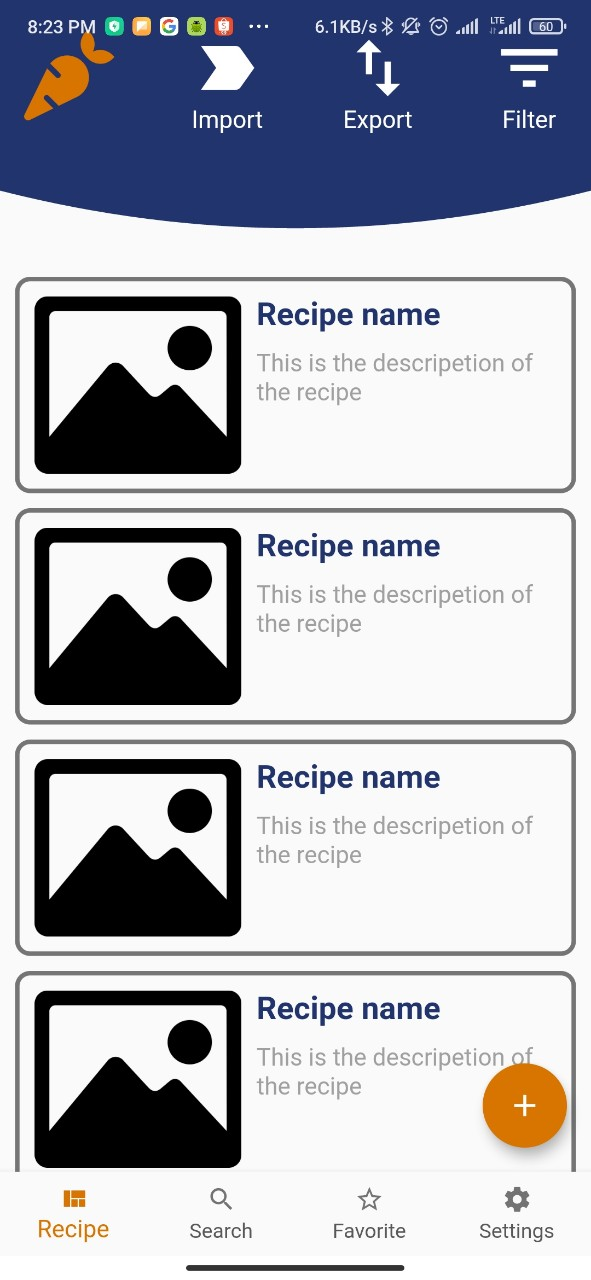
\includegraphics[scale=0.12]{Images/CookingBook.jpg}
    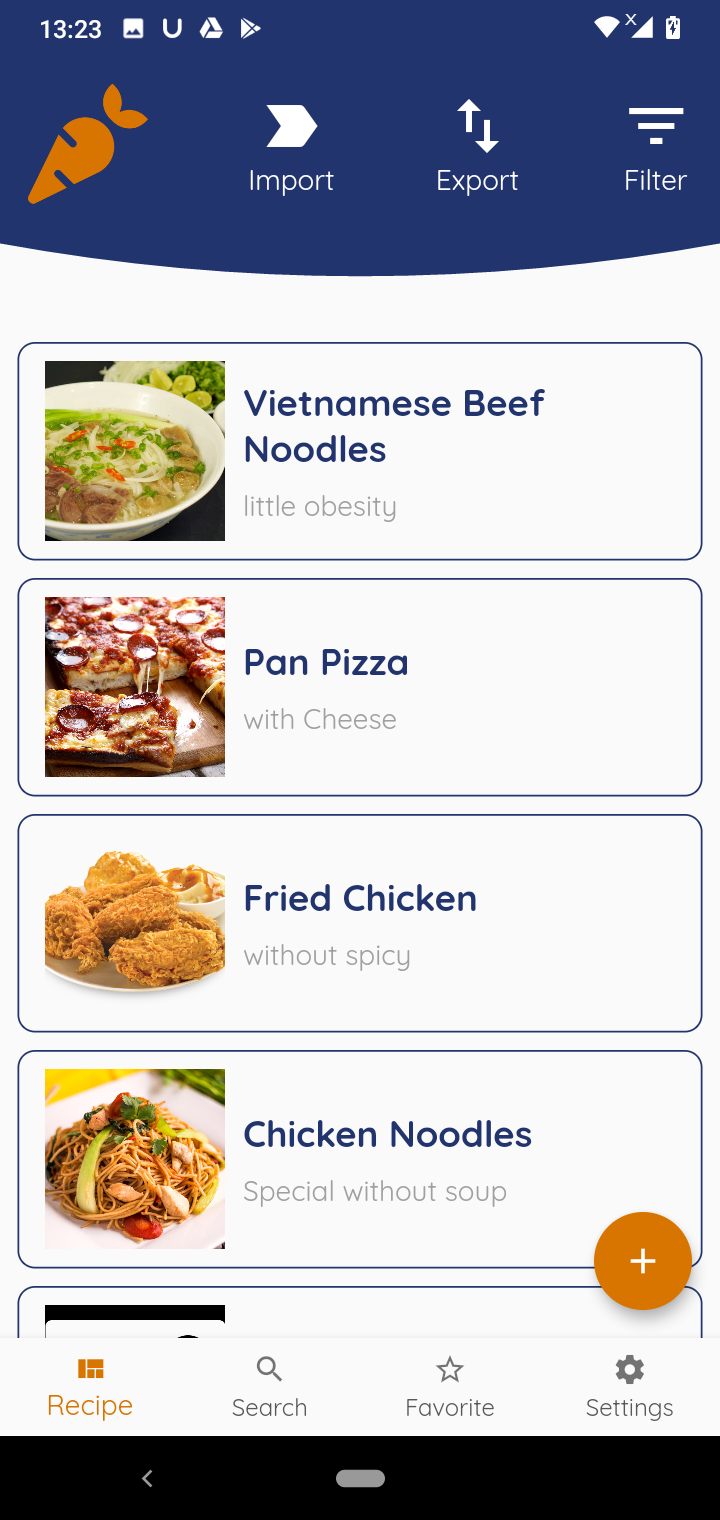
\includegraphics[scale=0.1]{Images/Home_interface.jpg}
    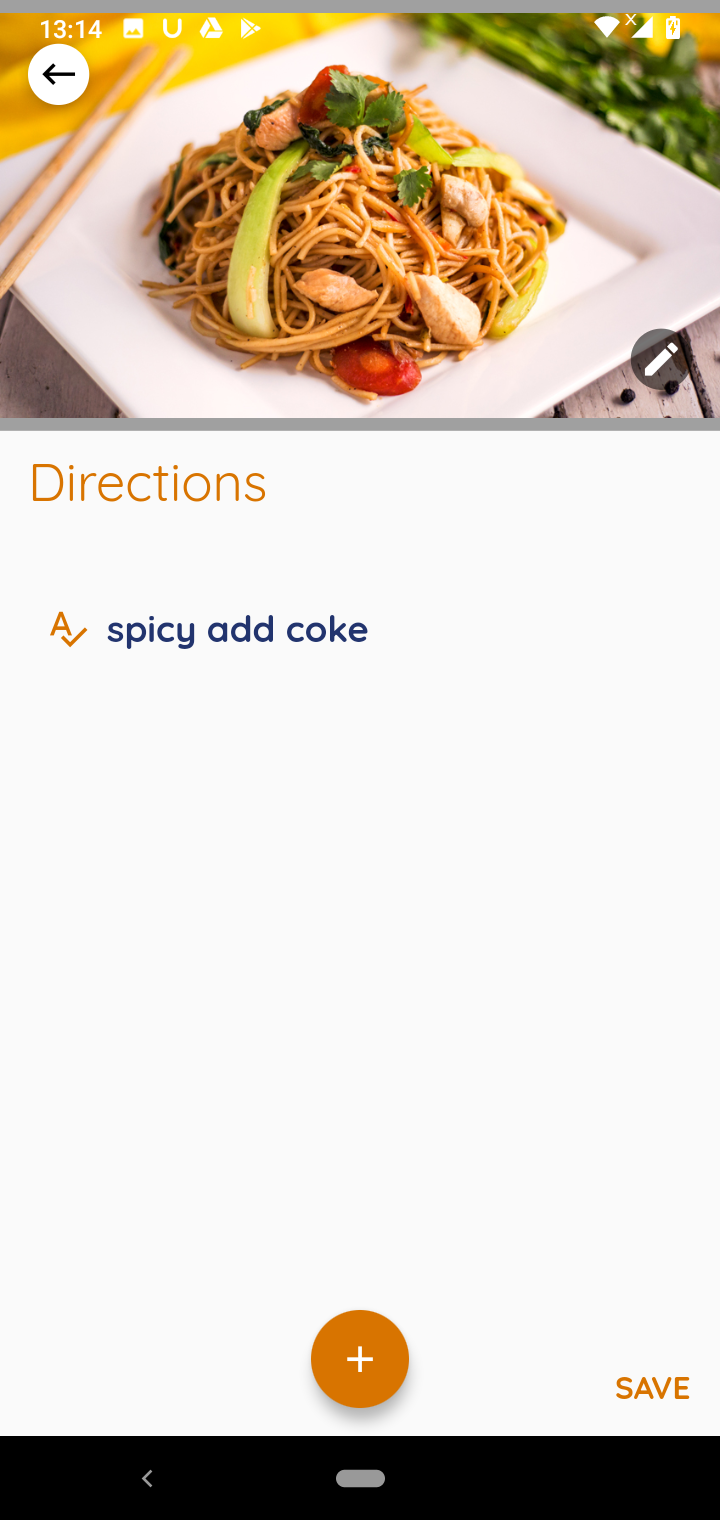
\includegraphics[scale=0.1]{Images/frienod_dire.jpg}
    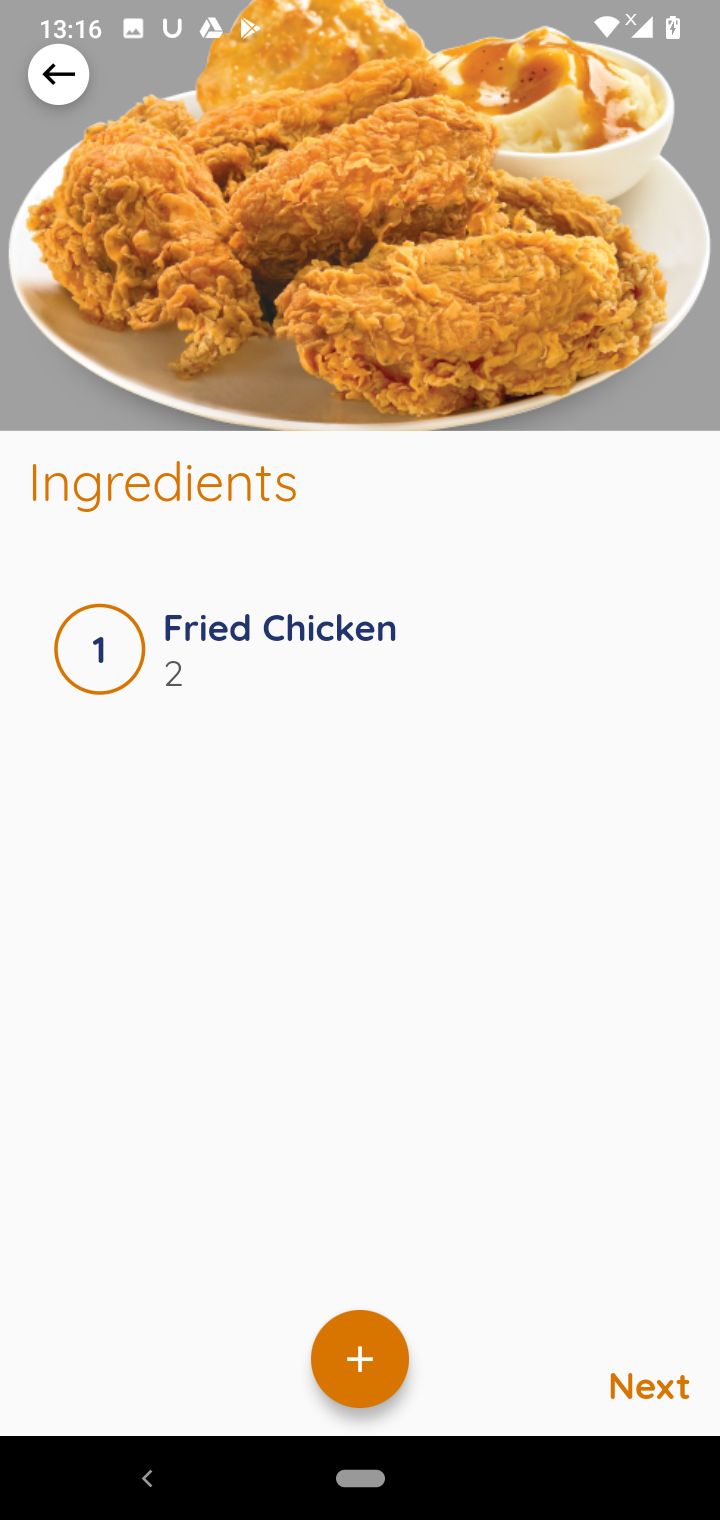
\includegraphics[scale=0.1]{Images/friechick_ingre.jpg}
    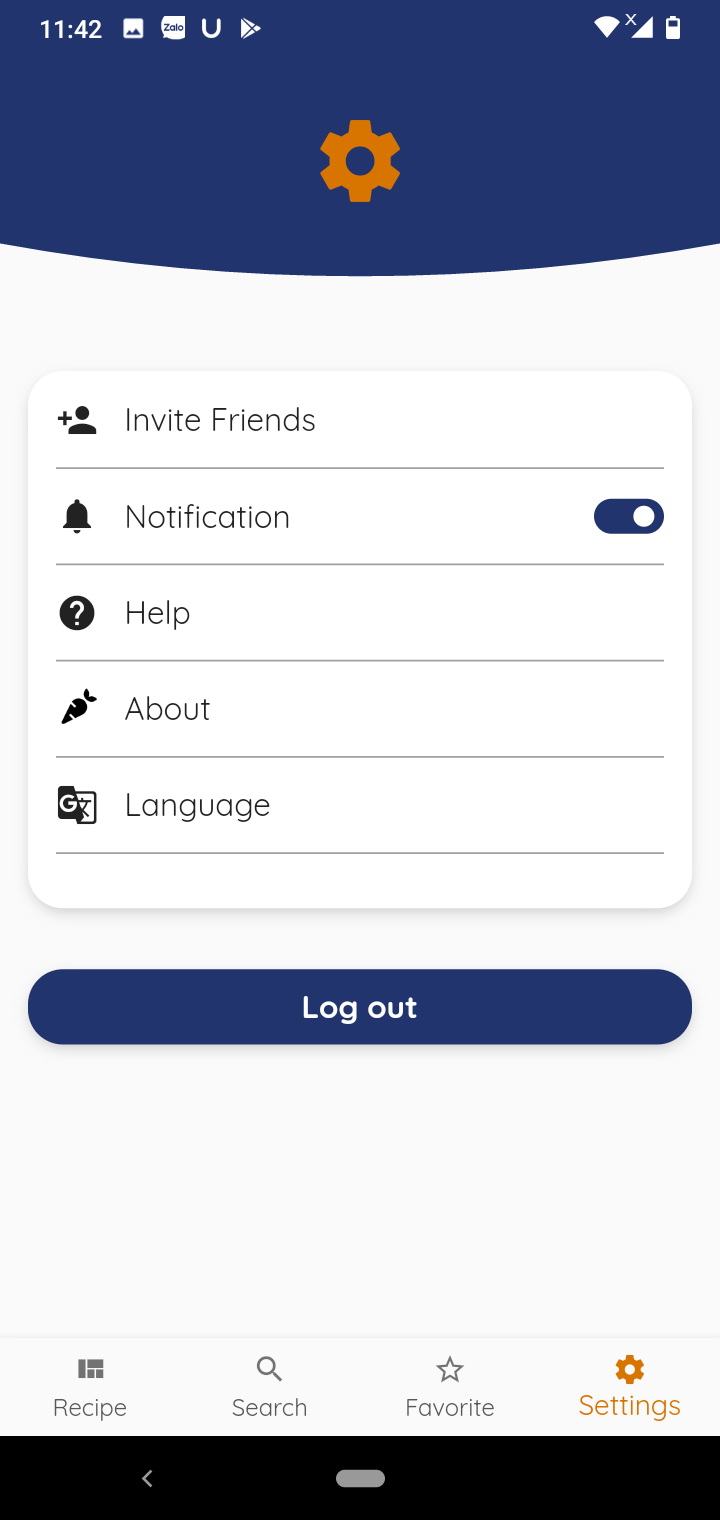
\includegraphics[scale=0.1]{Images/Settings.jpg}
    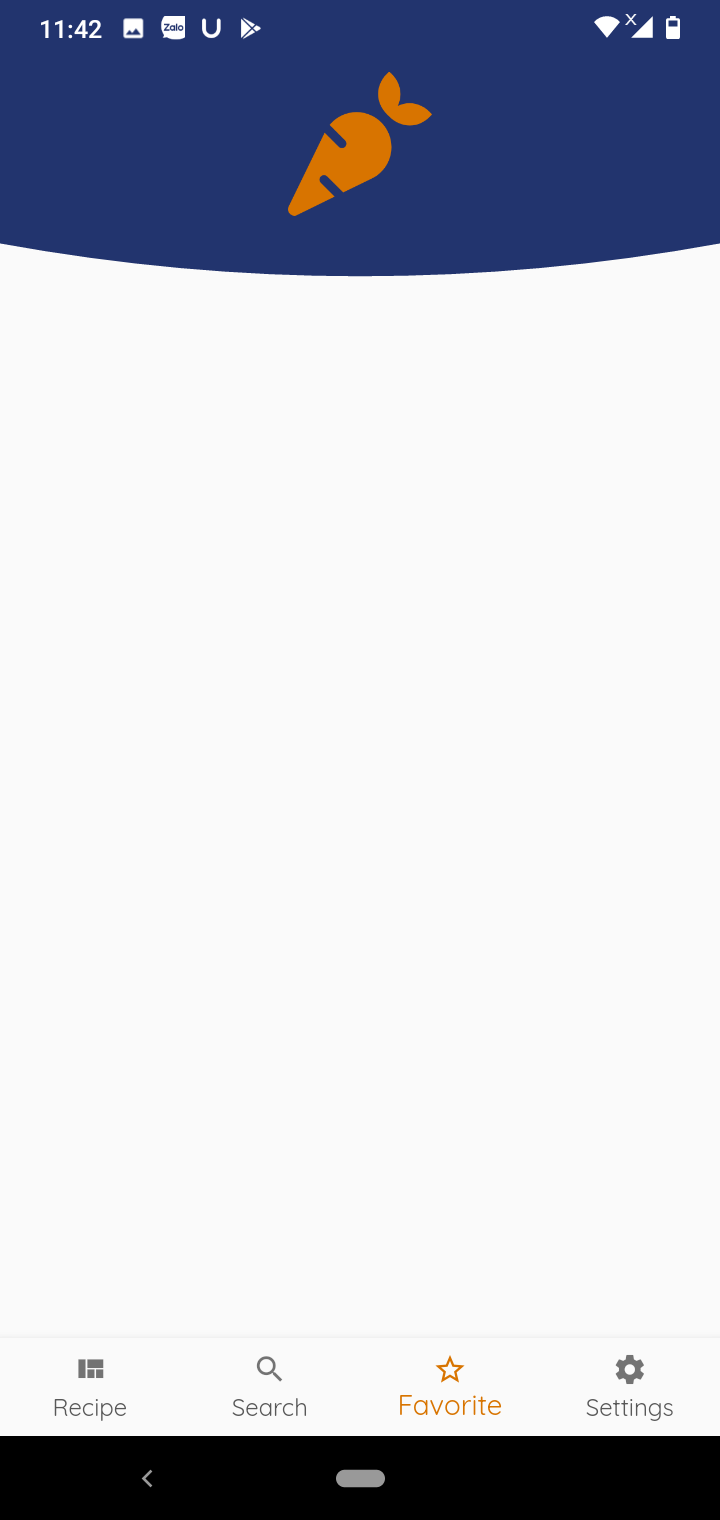
\includegraphics[scale=0.1]{Images/Favorite.jpg}
    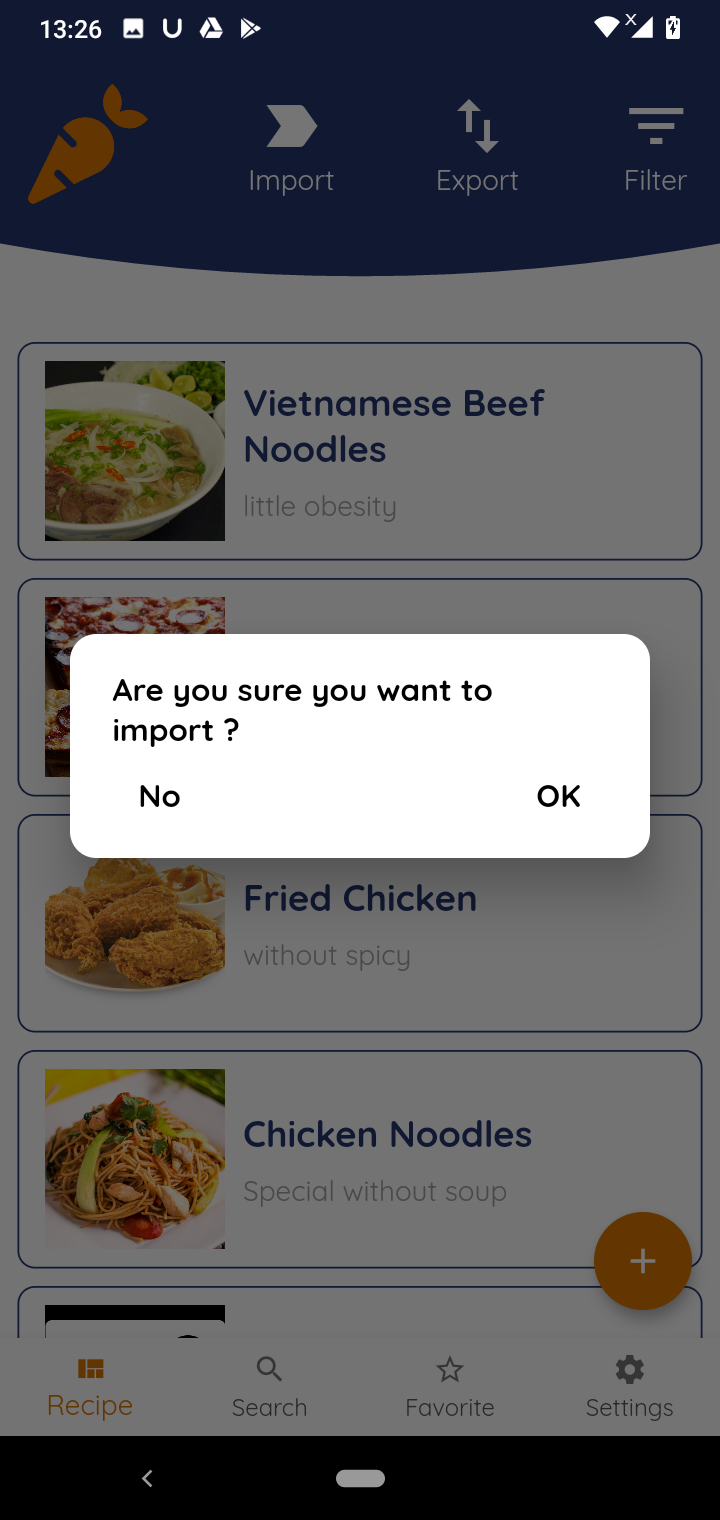
\includegraphics[scale=0.1]{Images/Import_annouce.jpg}
    \caption{Cooking Book App User Interface}
    \label{fig:cookingbook}
\end{figure}
\textbf{Download App and install}  \\
\begin{enumerate}
        \item \textbf{apk} for android Devices. under location /final/Cookbook.apk \href{/final/Cookbook.apk}{file} .
        \item \textbf{api} for IOS devices.
\end{enumerate}
\subsection{Application Demo}
Youtube Videos : \href{https://youtu.be/vgawyQmJWpk}{Application Demo}
\subsection{Source and github repository }
Github : \href{https://github.com/thphuc/cooking-app }{Git Url}


\newpage
\section{Project Details }
\subsection{Project Requirement}
\qquad The goal of this project is to have an app on the phone to handle our own recipes. It should be able to replace our handwritten recipe book while using smartphone abilities to add smart features.
\subsection{EXISTS ANALYSIS}
\qquad Analyze from similar applications and traditional recipe books that people use a lot today for business analysis, then give a comparison table below.
\begin{itemize}
\item Recipe book : Recipe books are easy to find at bookstores, like Magnolia Table Joanna Gaines.
\item Recipe website : Website of recipes, we can search, and get the recipe on this website. ex : \href{https://allrecipes.com}{All Recipes}.
\item Recipe App : But the recipe manager app, we can use these apps on our phones, and don't need internet. ex : My cook book manager .
\item Recipe online app. : Application for management, social network for sharing recipes. ex : Tasty .
\end{itemize}
\begin{center}
 \begin{tabular}{||c c c c c||} 
 \hline
  & Recipe Book & Recipe Website & Recipe App & Recipe Online App \\ [0.5ex] 
  & (Magnolia Table) & (\href{https://allrecipes.com}{All Recipes}) & (My cook book manager) & (Tasty) \\ [0.5ex] 
 \hline\hline
My own recipe & No & No & Yes & Yes \\ 
 \hline
 Search recipe & No & yes & yes & yes \\
 \hline
 easy to use & no & no, need account & yes & yes \\
 \hline
 cost & costly & free & free &  costly\\
 \hline
 internet & No & Require & no & Require \\ [1ex] 
 \hline
 Mobile Use & No & Yes, Require Internet & Yes & Yes \\ [1ex] 
  \hline
 Favorite & No & no, need account & Yes & Yes \\ [1ex] 
 \hline
  Import, Export & No & no & yes & no \\ [1ex] 
 \hline
\end{tabular}
\caption{Table 1.Compare kind of existing cook book}
\end{center}
\newpage
\subsection{Software Development}
\subsubsection{ARCHITECTURE}  \\ \\ 
\textbf{*Overall architecture} \\
\begin{figure}[h!]
    \centering
    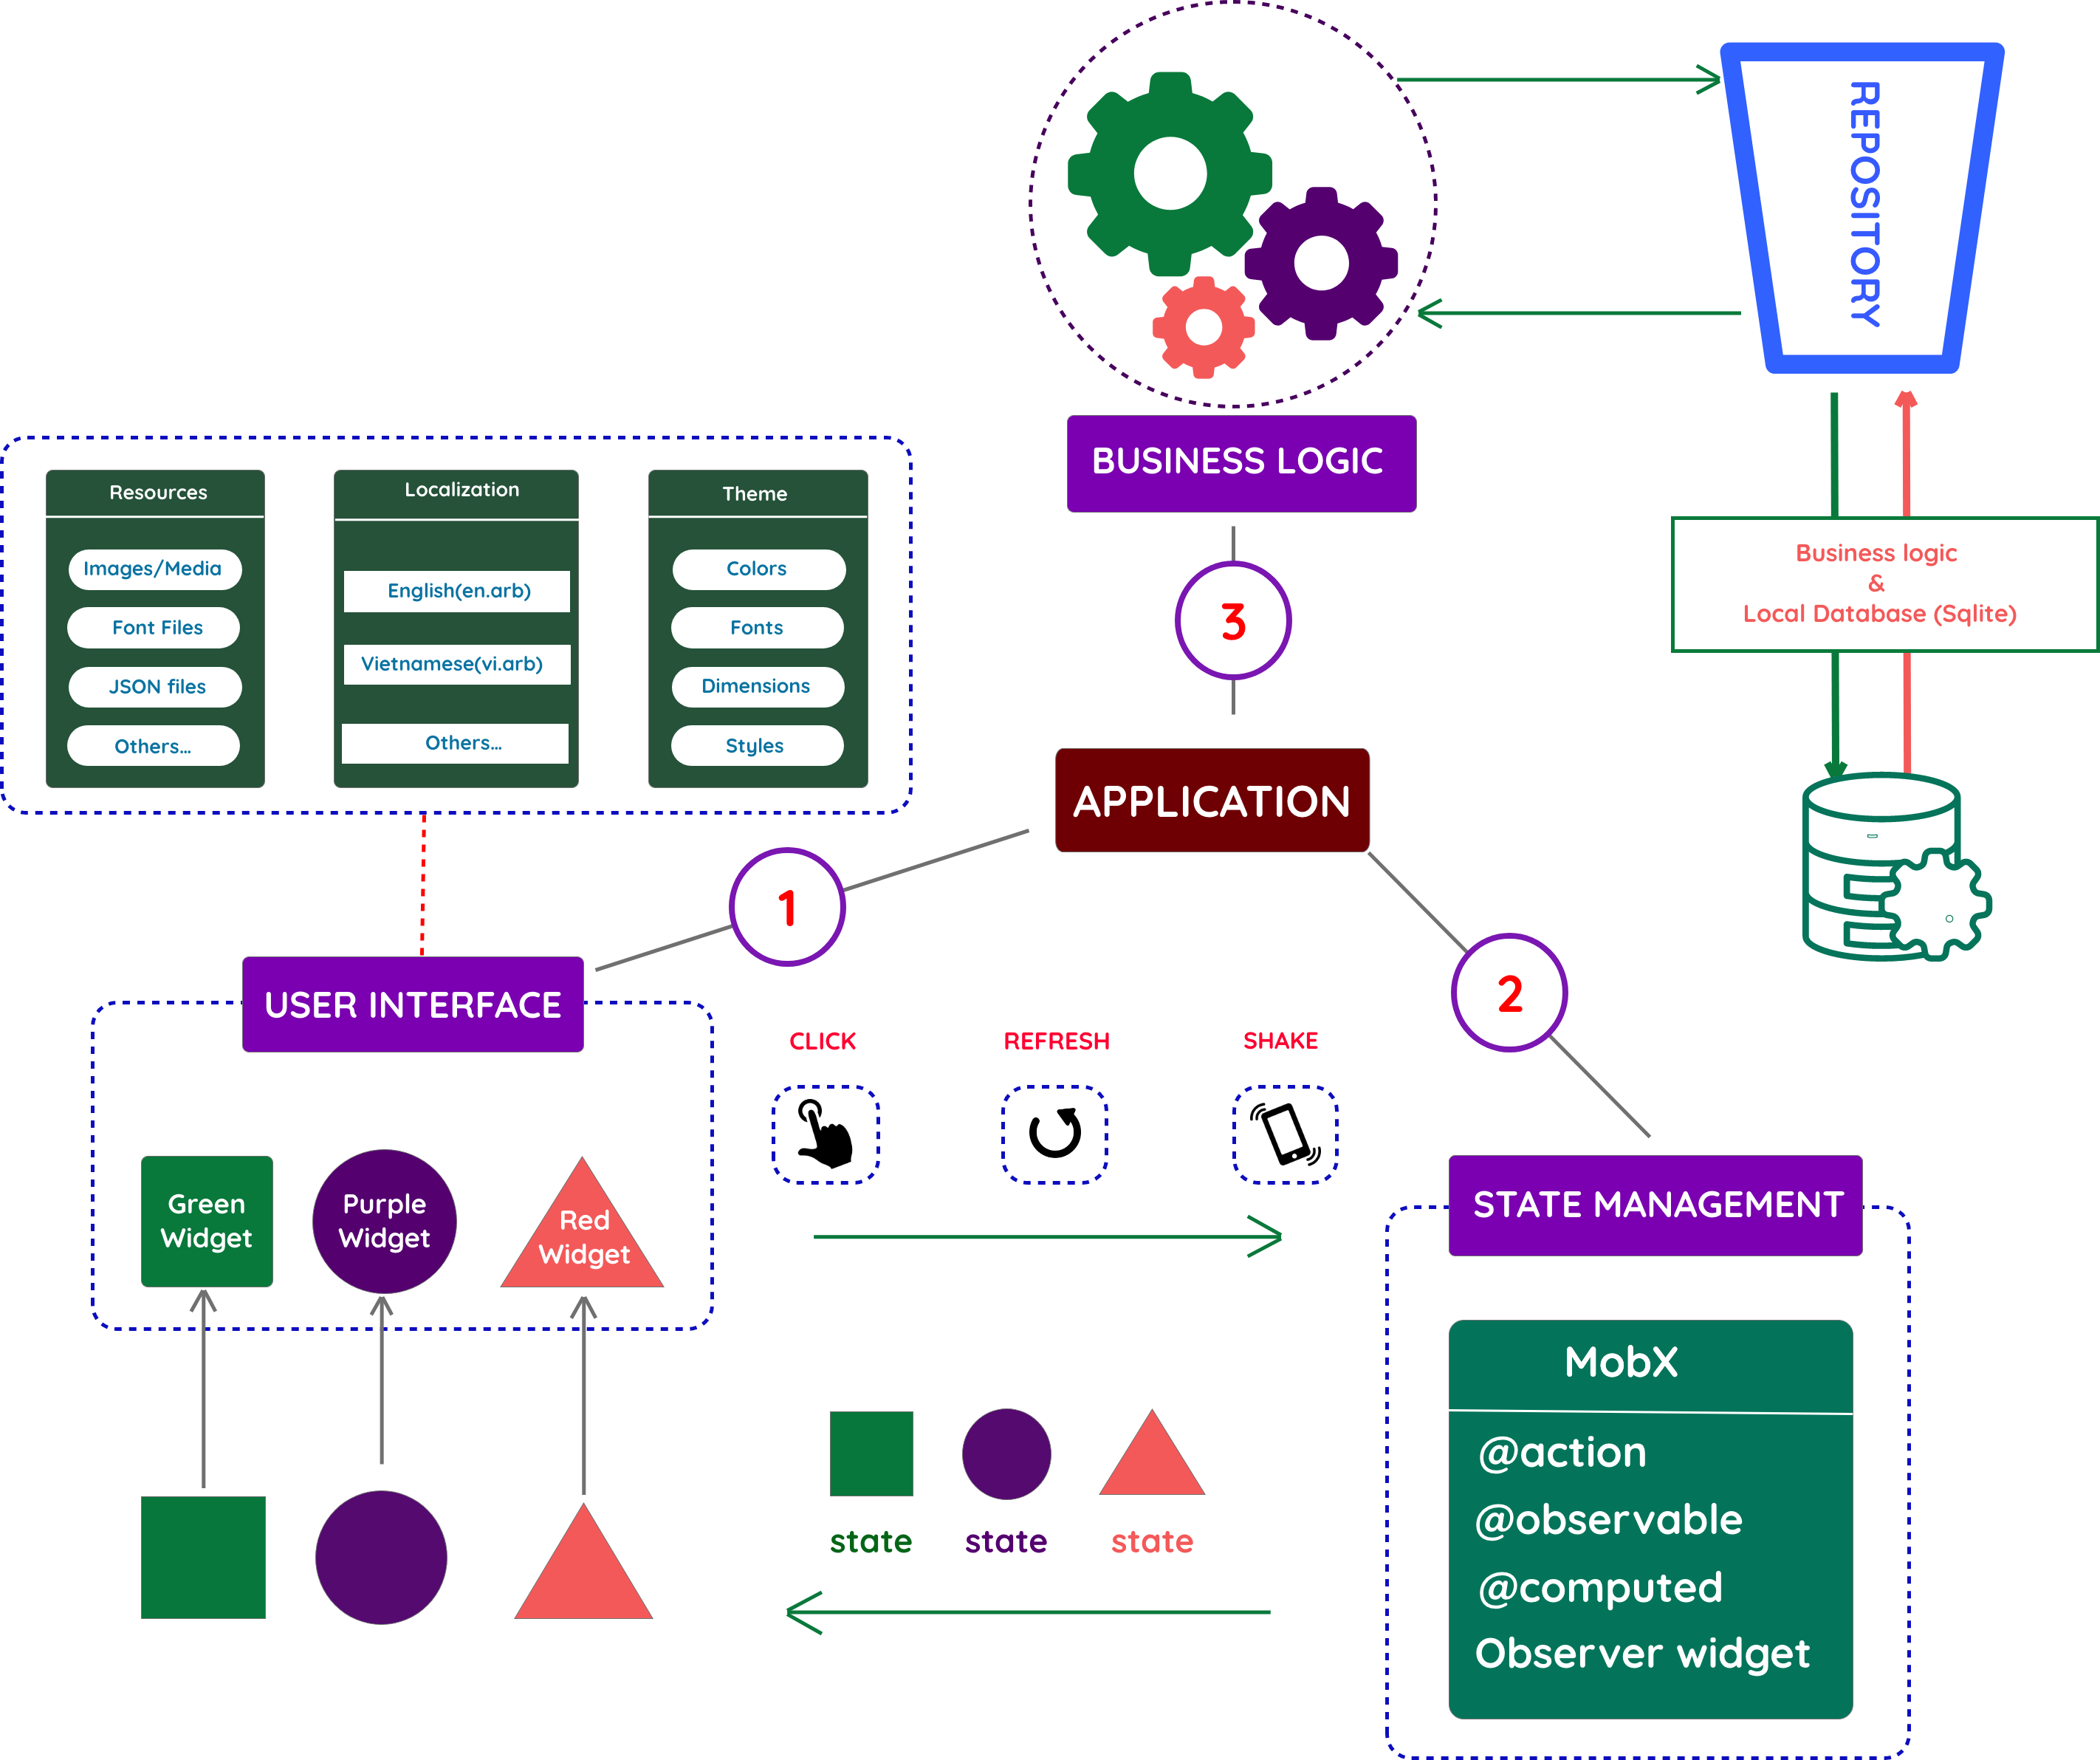
\includegraphics[scale=0.11]{Images/app-architecture.png}
    \caption{The overall architecture of the application}
    \label{fig:cookingbook}
\end{figure}

\textbf{*Components} :
    \begin{enumerate}
        \item \textbf{User Interface} : A place to display information to users, and to handle events on the user's side - interactive with smart phone devices, included UI ( Display User Interface), Resource ( Images, json file store, v.v.. ), Localization (Resource file for translation data store in smart devices ) Themes ( Color, Front, Dimensions, Styles , v.v... ). 
        \item \textbf{Business Logic } : Business logic layer and business layer, to process business information from users, or to interact with the database. Included Repository - business logic process components for recipe and related.
        \item \textbf{ State Management } 
    \end{enumerate}
\newpage
\subsubsection{IMPLEMENTATION CHOICES} : \\ \\
\textbf{*Programming language} :\\
Dart is the programming language we will use.

"Dart is a client-optimized[8] programming language for apps on multiple platforms. It is developed by Google and is used to build mobile, desktop, server, and web applications.[9] \\
Dart is an object-oriented, class-based, garbage-collected language with C-style syntax.[10] Dart can compile to either native code or JavaScript. It supports interfaces, mixing, abstract classes, refiled generics, and type inference.[11]"* \\
\href{https://en.wikipedia.org/wiki/Dart_(programming_language)}{By Wikipedia.}\\\\
Dart is very powerful when combined with Flutter in developing cross-platform mobile applications, and that why team decides to use the combo Dart and Flutter to develop the mobile Application.
Dart and Flutter has the growth rate is very fast in recent years.

\begin{figure}[h!]
    \centering
    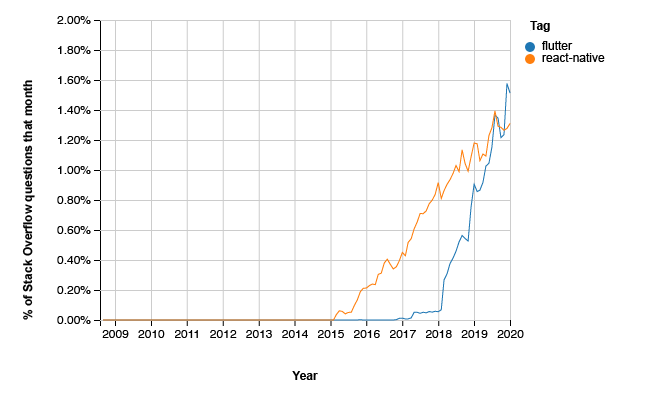
\includegraphics[scale=0.7]{Images/MobileTrend.png}
    \caption{Stack Overflow Trends — Comparison of Flutter vs. React Native}
    \label{fig:cookingbook}
\end{figure}
*Source : \href{https://insights.stackoverflow.com/trends?tags=flutter,react-native}{Stackoverflow Insight} \\
\textbf{*Framework}: \\\\
\textbf{Front-end (Mobile app) } \\
\qquad We only consider cross-platform frameworks: \href{https://reactnative.dev}{ React Native} or  \href{https://flutter.dev}{Flutter}. The reasons behind this decision are:
 \begin{enumerate}
        \item After analyzing the requirements (both non-functional and functional requirements), we concluded that the application does not require any specific native function that cross-platform framework can not do.
        \item We don’t have enough time and resources to build and maintain 2 separate code bases (one for Android and one for iOS)
\end{enumerate}
\begin{figure}[h!]
    \centering
    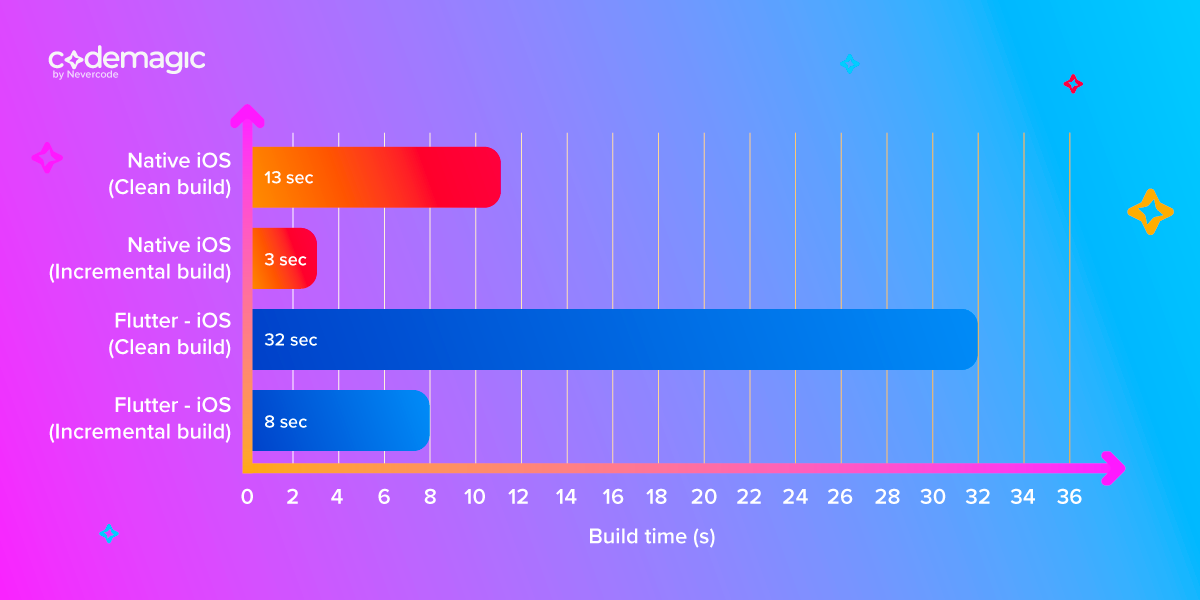
\includegraphics[scale=0.3]{Images/CM_Swift-vs-Flutter_build-time.png}
    \caption{Flutter vs native application comparison time}
    \label{fig:cookingbook}
\end{figure}
*Source : \href{https://blog.codemagic.io/flutter-vs-swift/}{Codemagic} \\\\


After we finished our research (visit their official website and documentation, read many articles (listed in references 4a. at the end of this document)), we ended up to choose Flutter for this project, because:
\begin{enumerate}
        \item Flutter has better performance(even better native in a few cases).
        \item Flutter has better documentation.
        \item Flutter is being developed and maintained by Google officially, while React native is not supported officially by Facebook anymore.
        \item Flutter will support web and PC(and probably other platforms in the future). 
\end{enumerate}

\textbf{References}
\begin{enumerate}
\item https://www.thedroidsonroids.com/blog/flutter-vs-react-native-what-to-choose-in-2020 
\item https://nevercode.io/blog/flutter-vs-react-native-a-developers-perspective/
\item https://medium.com/@adhithiravi/react-native-vs-flutter-what-are-the-differences-b6dc892f0d34
\item https://medium.com/@moqod-development/flutter-vs-react-native-for-cross- platform-development-821b44138b4a
\item https://medium.com/swlh/flutter-vs-native-vs-react-native-examining-performance- 31338f081980
\item \textbf{Flutter documentation: }  https://flutter.dev/docs
\end{enumerate}

 \subsubsection{LISIBITLY} : in cooking app, we included : 
 \begin{enumerate}
 \item : Analyzer for Dart to check rule of code, or comment, v.v...
 \item : Dartdoc : To generate document of Dart programming language code. Docs api at location : /final/source_code/doc/api/* \href{/final/source_code/doc/api/}{Location }
 \end{enumerate}
 \begin{figure}[h!]
    \centering
    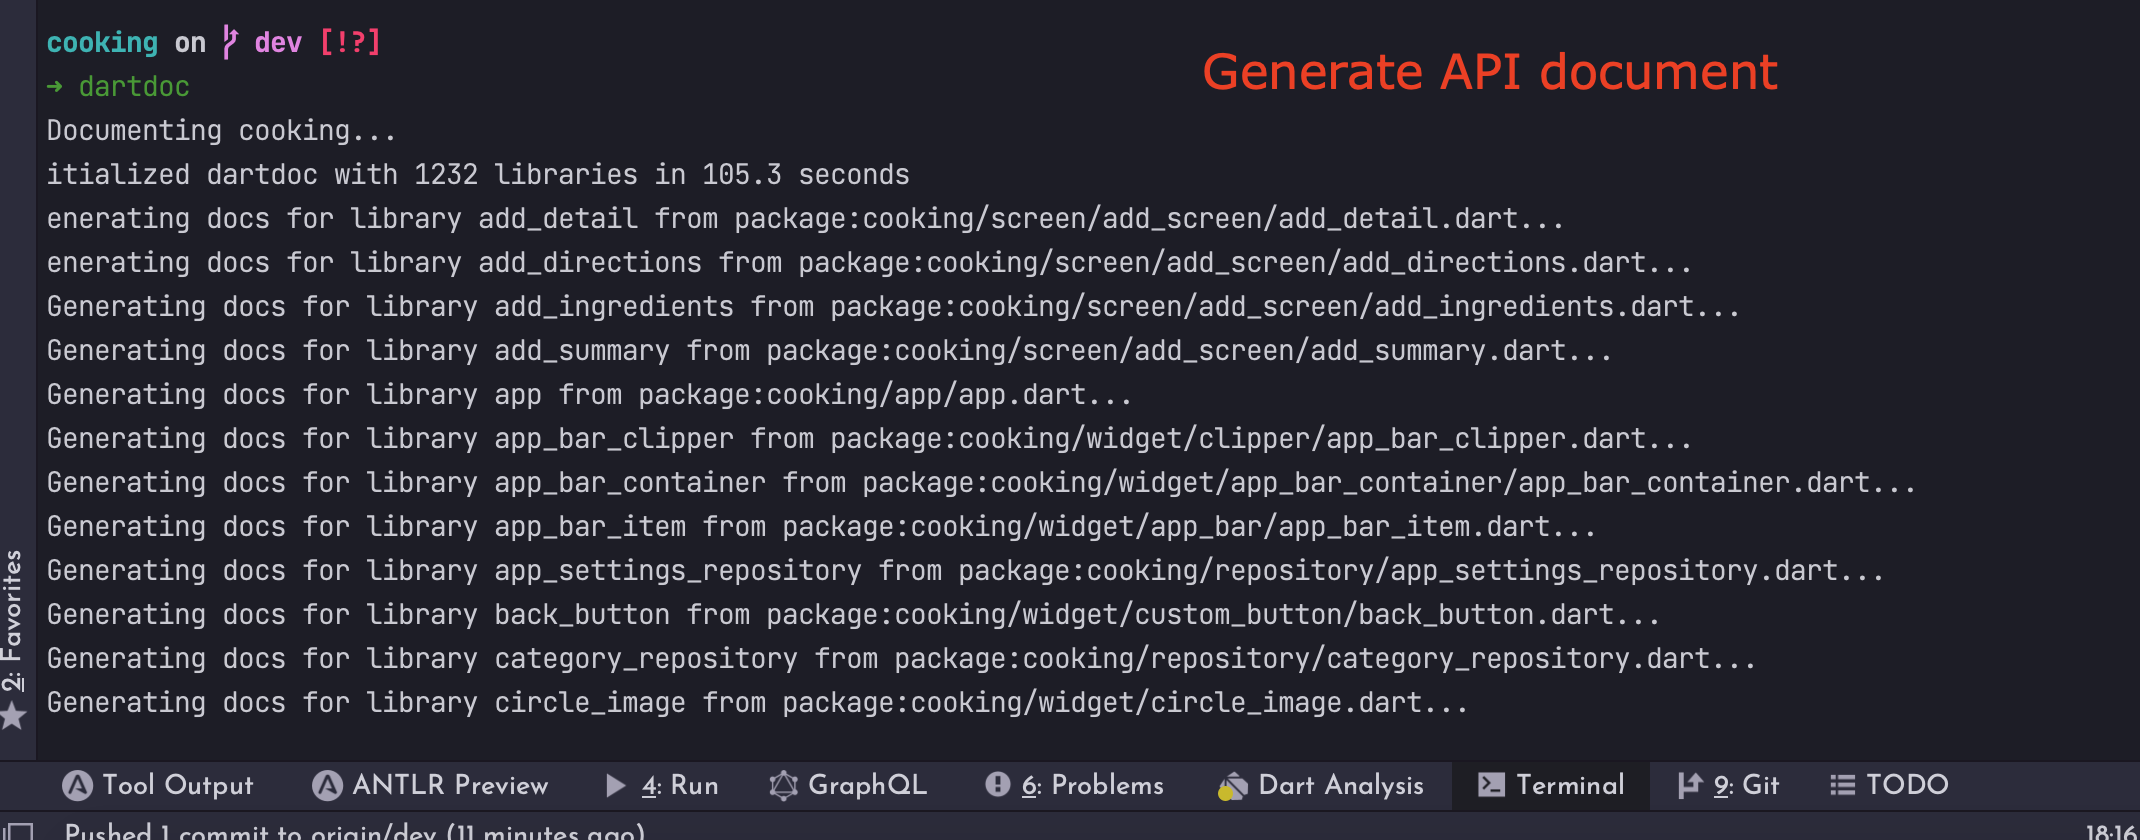
\includegraphics[scale=0.25]{Images/generatedoc.png}
    \caption{Generate Document}
    \label{fig:cookingbook}
\end{figure}

 \begin{figure}[h!]
    \centering
    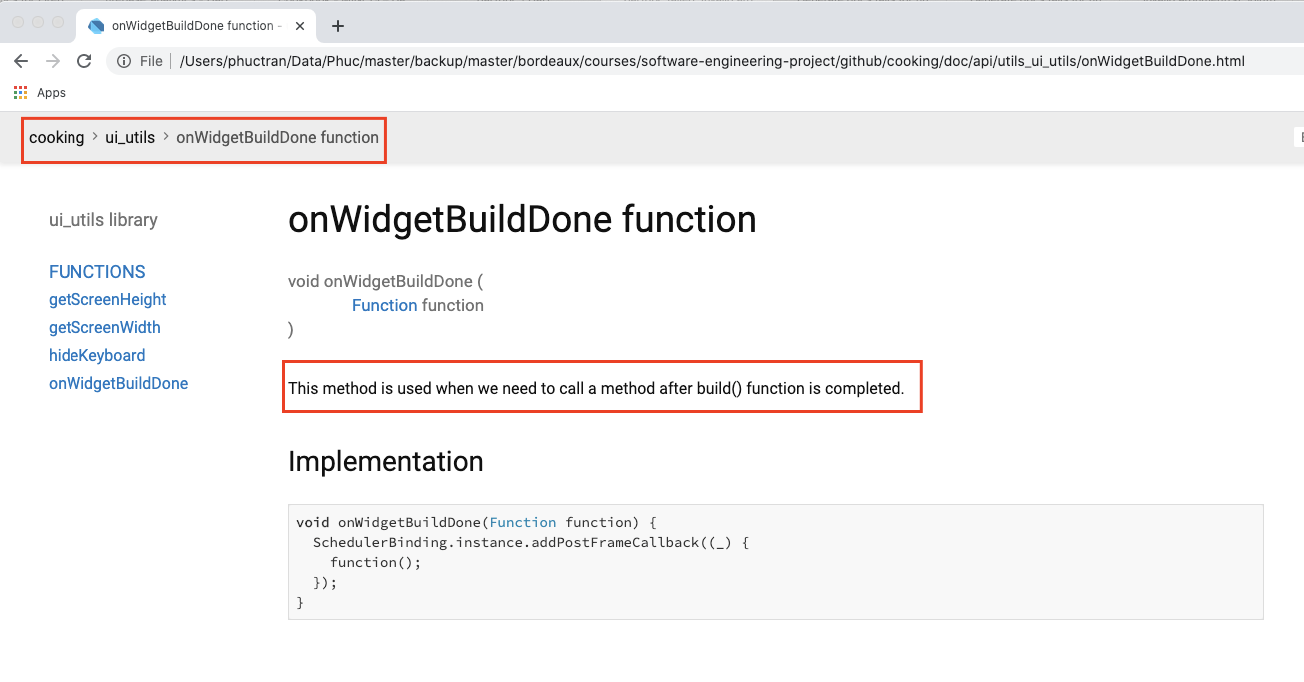
\includegraphics[scale=0.30]{Images/docapi.png}
    \caption{After generate, it should document api}
    \label{fig:cookingbook}
\end{figure}

 \begin{figure}[h!]
    \centering
    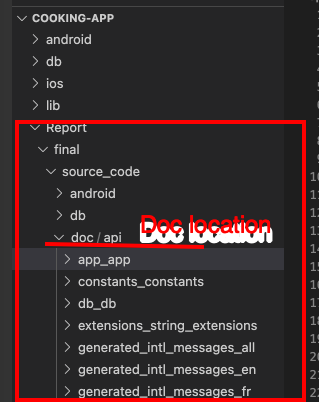
\includegraphics[scale=0.6]{Images/doc_location.png}
    \caption{Doc Location Under /final/source_code/doc/api/*}
    \label{fig:cookingbook}
\end{figure}

 \subsubsection{ROBUSTNESS}  :  in cooking app, we included : 
 \begin{enumerate}
 \item Unit-test : Unit test for repository - business layer of recipe and recipe categories, when every time we have new code, we can re-run the whole unit code to make sure the system still working fine with Mock data.
 \item Log : We use fire-base to log error/exception .
 \end{enumerate}
 \begin{figure}[h!]
    \centering
    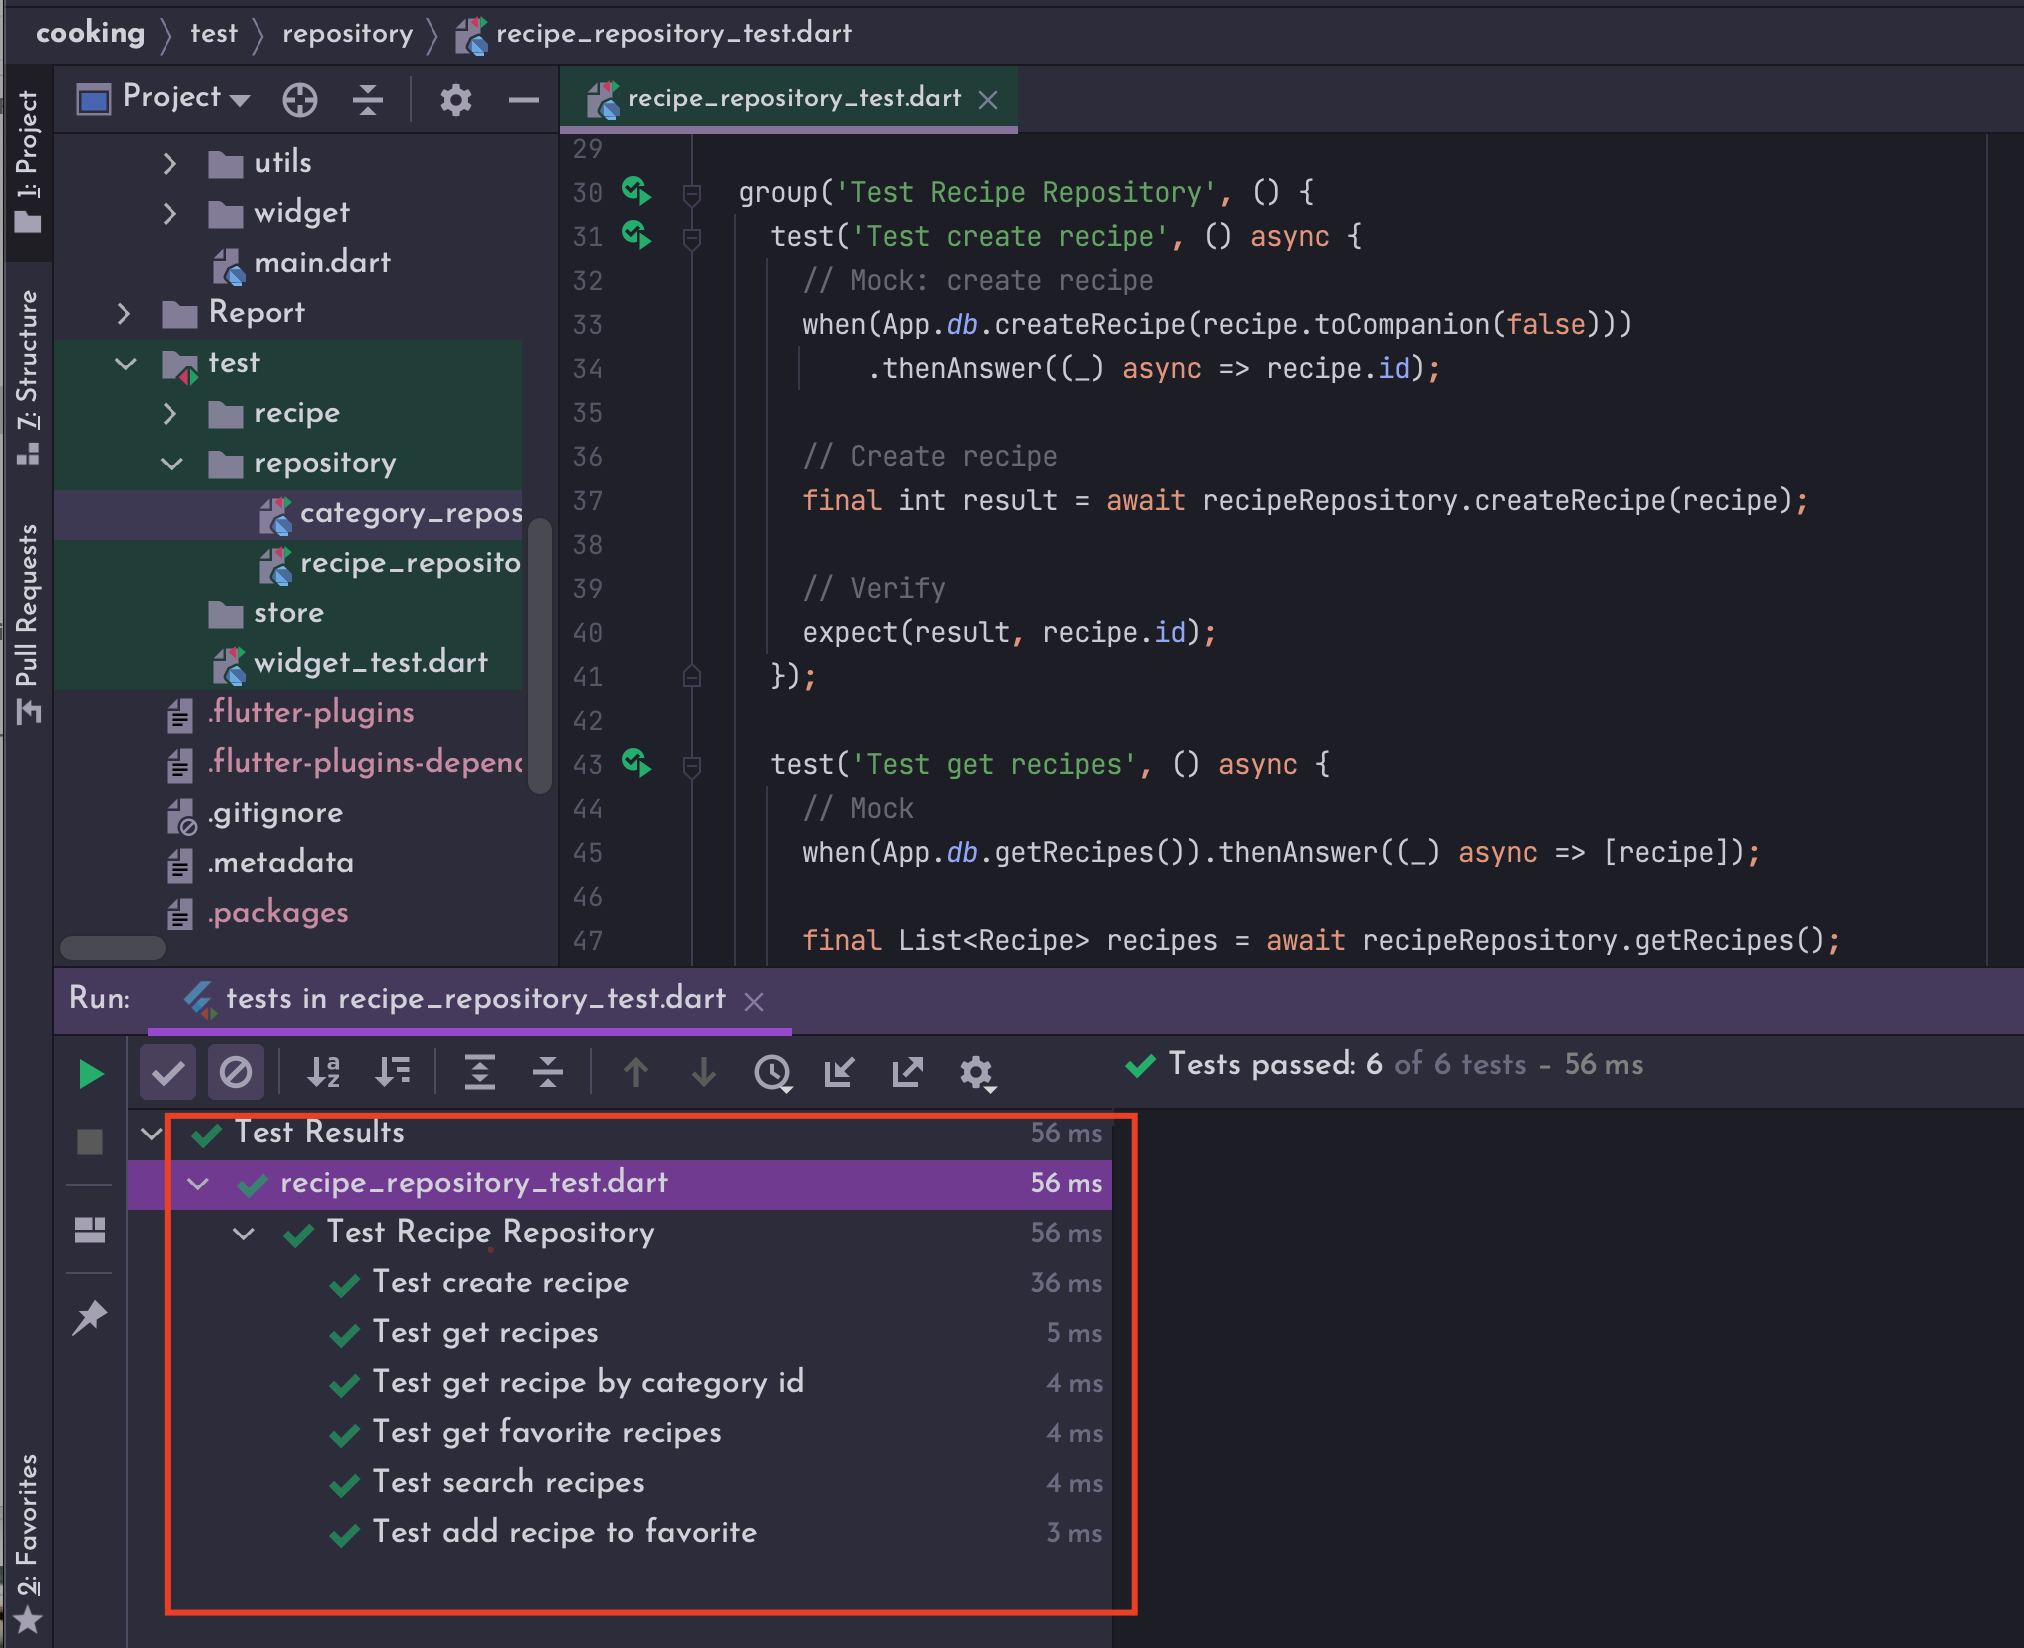
\includegraphics[scale=0.2]{Images/unit-test-repo.png}
    \caption{Unit-test of repository (all passed)}
    \label{fig:cookingbook}
\end{figure}
\begin{figure}[h!]
    \centering
    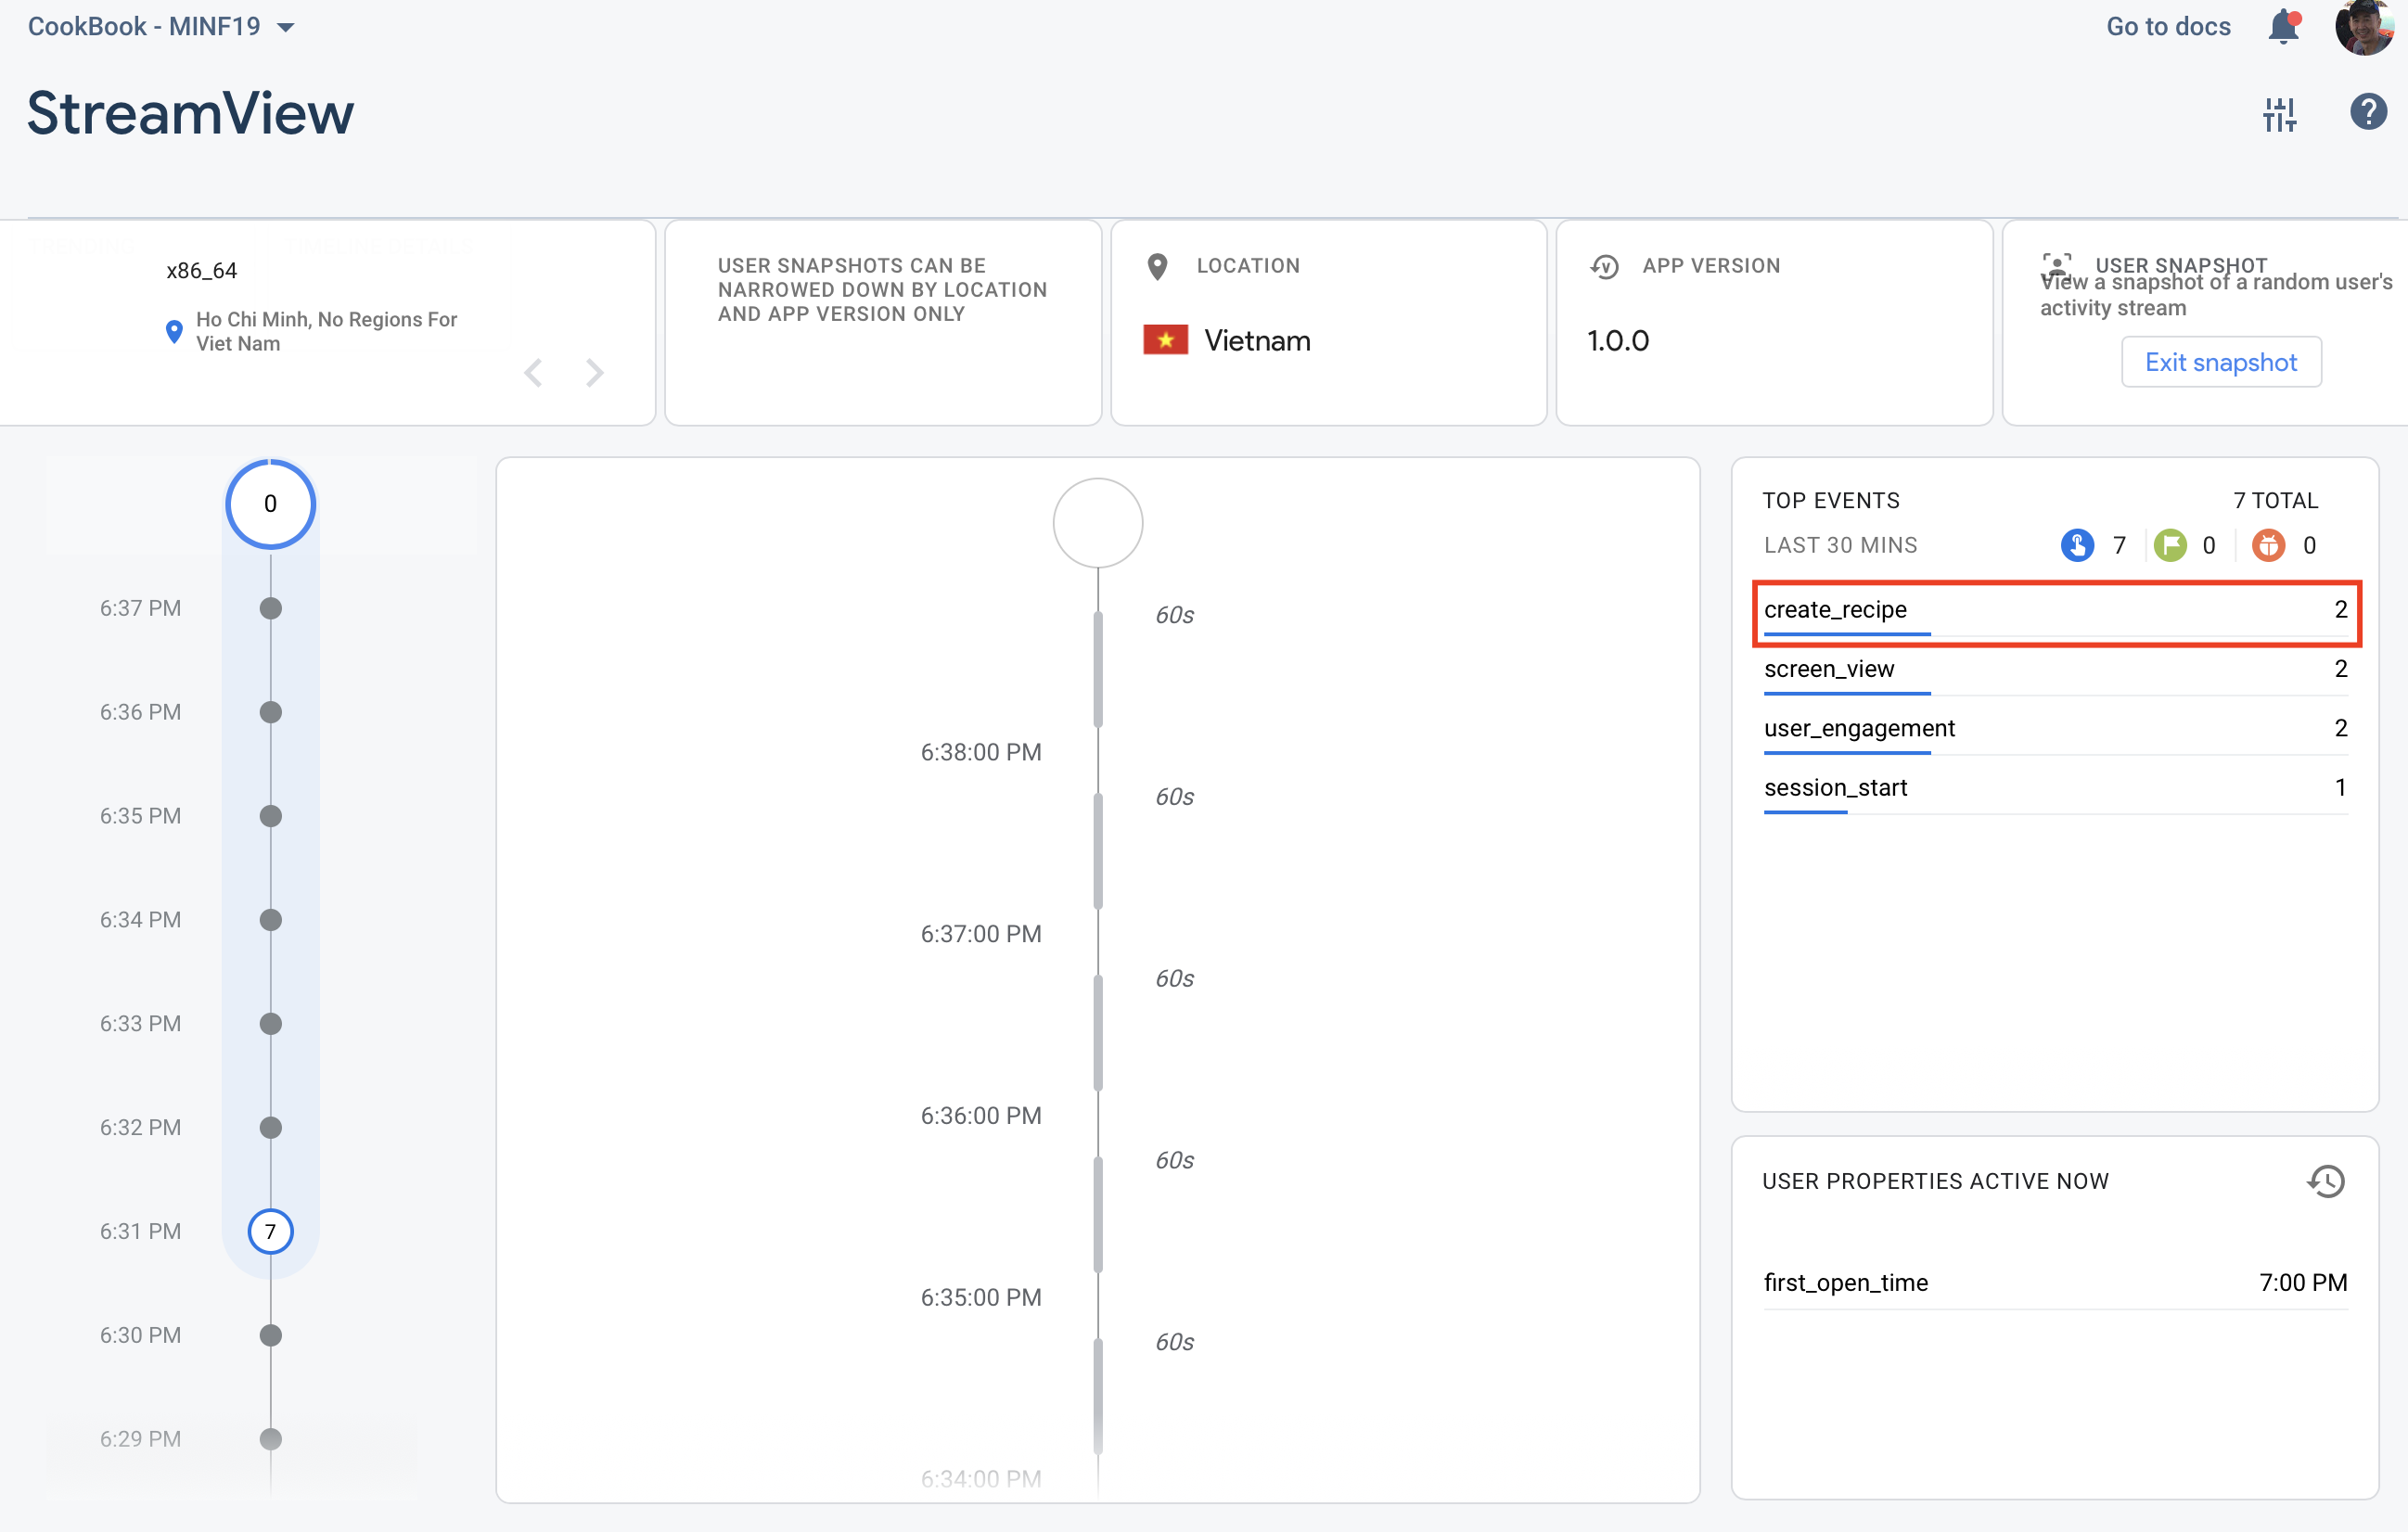
\includegraphics[scale=0.2]{Images/firebaselog.png}
    \caption{Fire-base for logging}
    \label{fig:cookingbook}
\end{figure}
\begin{figure}[h!]
    \centering
    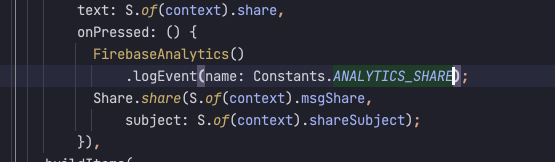
\includegraphics[scale=0.45]{Images/firebaselog-setup1.png}
    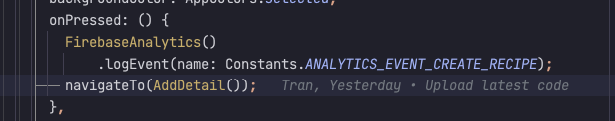
\includegraphics[scale=0.45]{Images/firebaselog-setup2.png}
    \caption{Setup Fire-base}
    \label{fig:cookingbook}
\end{figure}

\newpage
\subsubsection{REQUIREMENT ANALYSIS  }\\\\
\textbf{ *Use-case diagram}\\
\begin{figure}[h!]
\centering
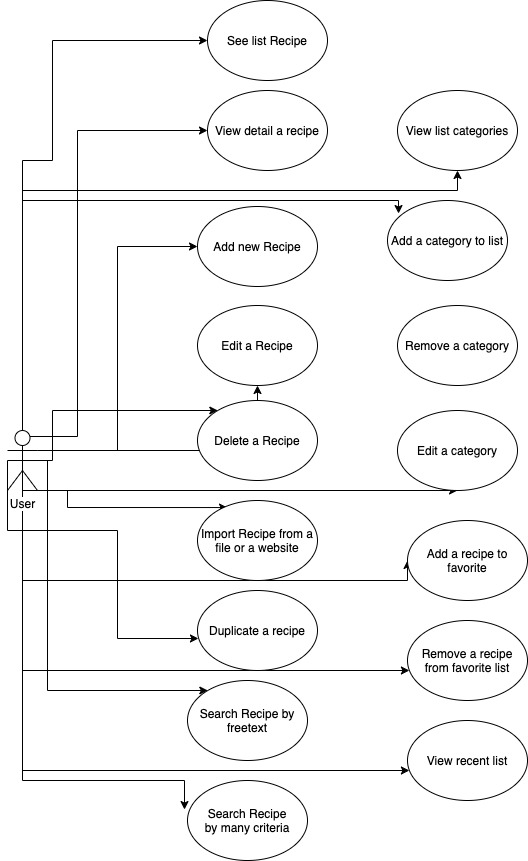
\includegraphics[scale=0.5]{Images/Usecase.jpg}
\caption{Use-case diagram}
\label{fig:Usecase}
\end{figure}
\newpage
\textbf{*Mock-up}
\begin{figure}[h!]
\centerin
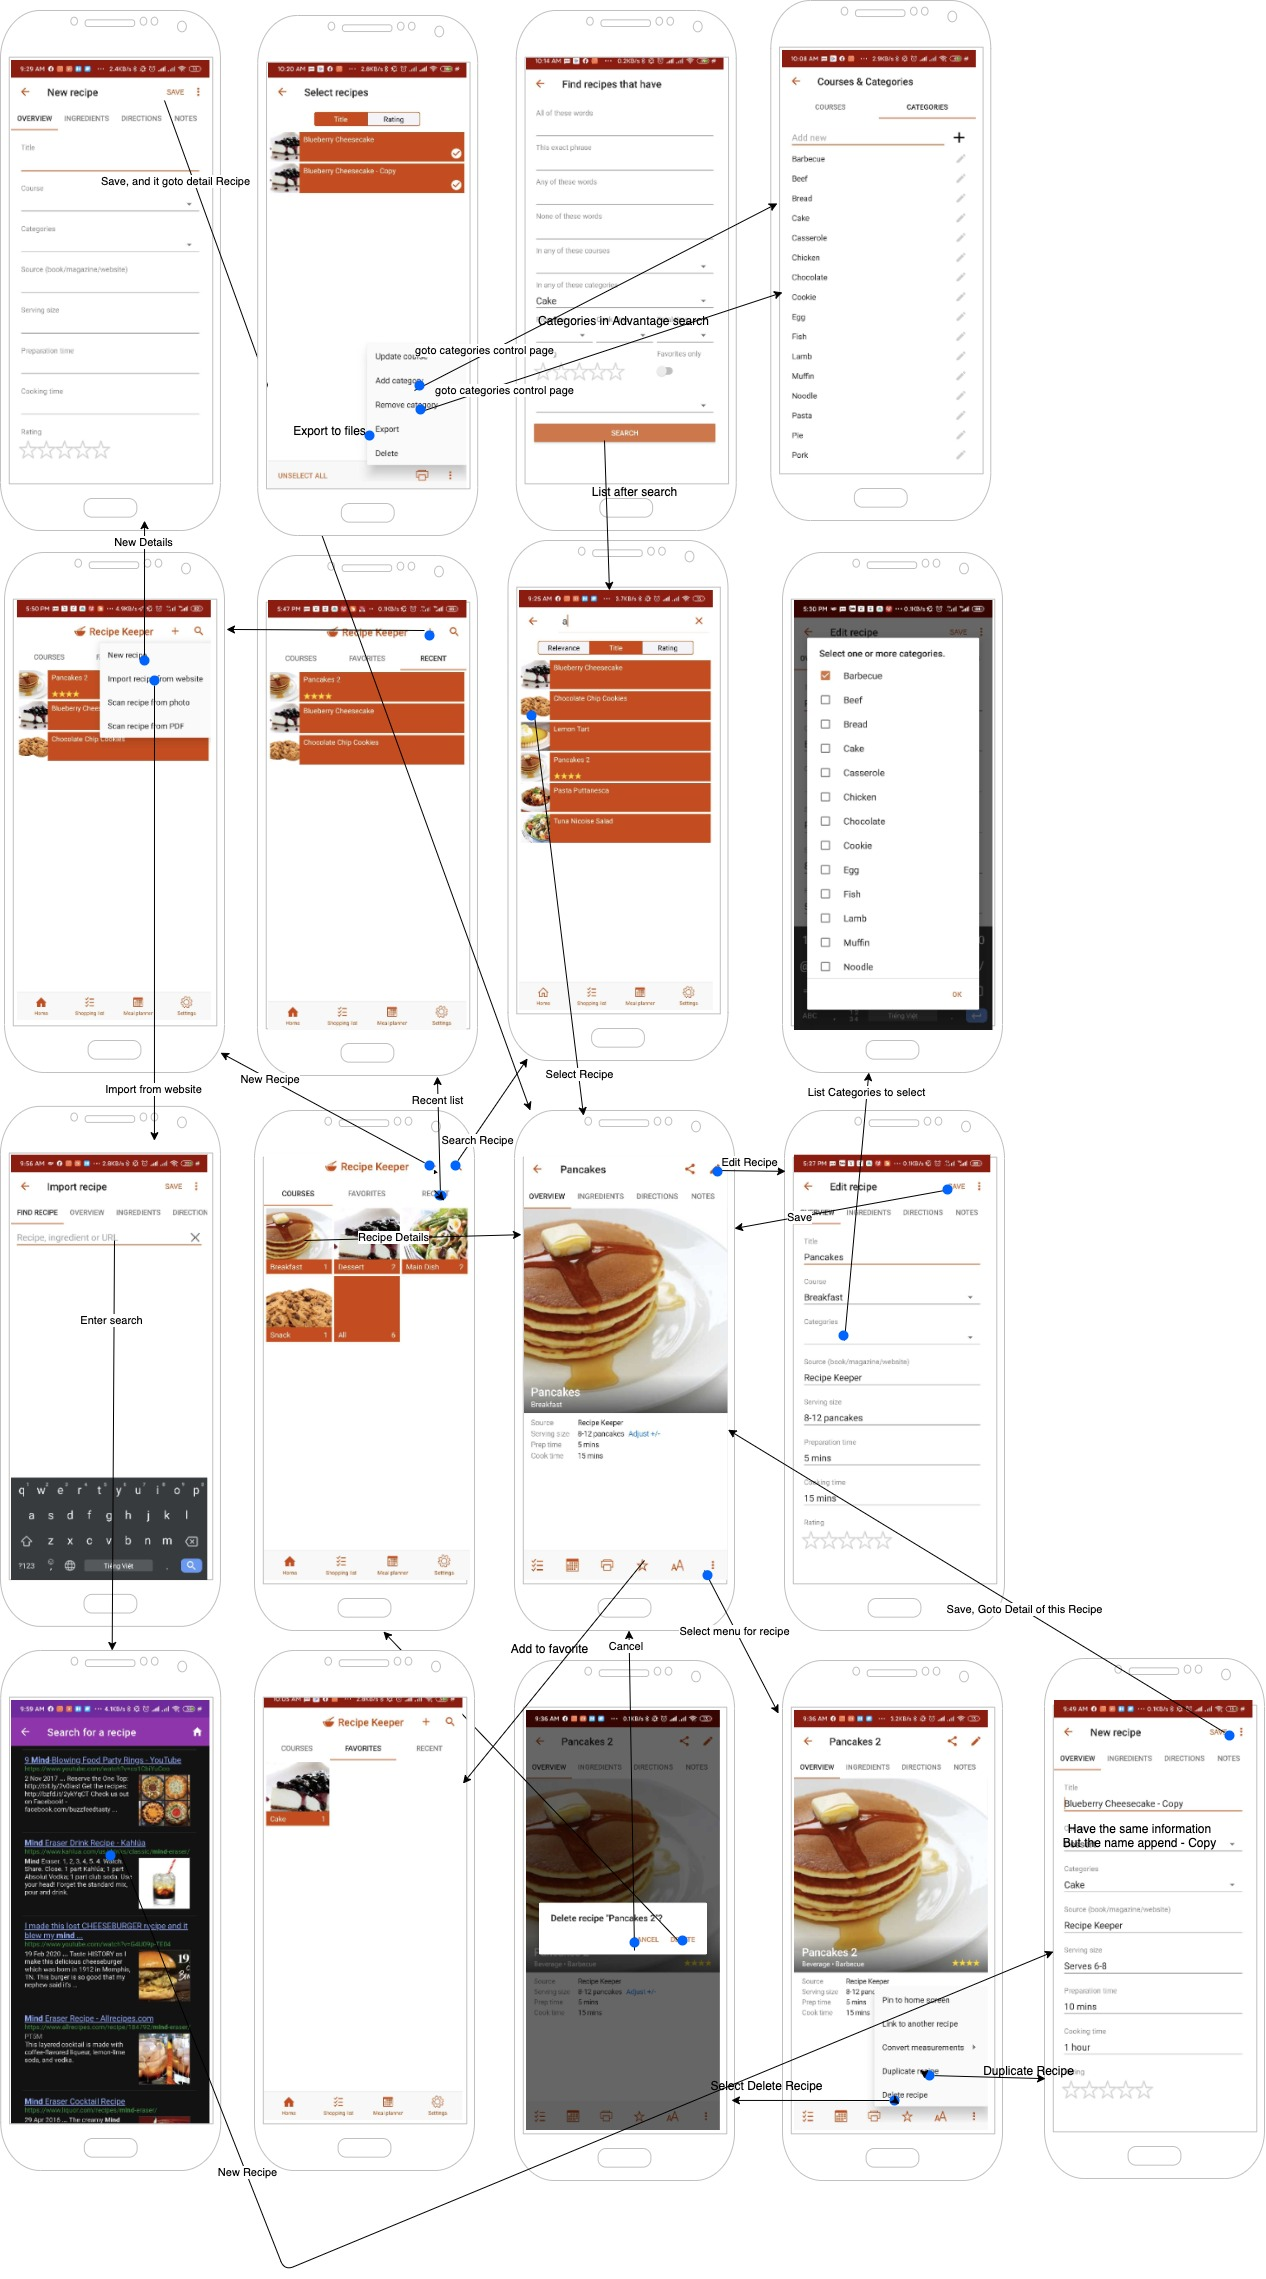
\includegraphics[scale=0.21]{Images/Mockup.jpg}
\caption{Mock-up UI and flow of app}
\label{fig:Mockup}
\end{figure}
\newpage
    \textbf{* Functional Requirement} : 
    \begin{enumerate}
        \item \textbf{Recipe list }:User can view their recipe list on homepage. Each item on the list shows recipe basic information (name, image, short description).
        \item \textbf{Sort recipes }: user can sort their recipes in different orders(Ex:name, created date), default order is name. 
        \item \textbf{Create new recipe} : user has the ability to create new recipe from the app.
        \item \textbf{View recipe details} : user can click on any recipe on the recipe list to view its details.
        \item \textbf{Edit recipe}: user is able to edit existing recipe and save updated details to database.
        \item \textbf{Delete recipe}: user can delete an existing recipe. A popup dialog should be shown to user to confirm the deletion. After deleted, the recipe will be removed our of local database and disappears on recipe list.
        \item \textbf{Duplicate recipe}: user can use this function to clone an existing recipe to new one quickly.
        \item \textbf{Import recipes}: user is able to use the app to import one or more recipes from the file that was exported before. User can import recipes from the internet too.
        \item \textbf{Export recipes}: from the app, user can export one or more recipes to a file. This file can be shared to other users or re-imported to the app later.
        \item \textbf{Search recipe(s)}: user can search recipe(s) from local database or remote database.
        \item \textbf{Category list}: user can view list of categories. Click on a category to view all the recipes belong to that category.
        \item \textbf{Create new category}: from the app, user can create new category (with name and description).
        \item \textbf{Edit category}: user is able to edit the information of category.
        \item \textbf{Delete category}: user is able to delete existing categories. A popup dialog should be shown to user to confirm the deletion. After deleted, the deleted category will no longer be shown in category list.
        \item \textbf{Favorite recipes}: user can add any recipe to favorite list, so that user can find these recipes faster.
        \item \textbf{Remove recipes out of favorite list}: user is able to remove recipes out of the favorite list. A popup dialog should be shown to user to confirm the removal.
        \item \textbf{Push notification}: user can receive notifications (if they allow)
        \item \textbf{Resume Application}: When they're an action with higher priority ( like phone call ), the application should pause, and resume all progress when the action is finished.
    \end{enumerate}
\\ \\ \\ \\ \\
    \textbf{* Non-Functional Requirement} : 
    \begin{enumerate}
        \item \textbf{Performance/Storage} : Storage of application if acceptance ( < 100Mb )
        \item \textbf{Performance/Response} : All local response action must < 1s.
        \item \textbf{Performance/Memory} : Memory of application if acceptance for an manage application ( < 100Mb Memory when running ).
        \item \textbf{Responsiveness}: with any “unexpected event” from user, like a phone call, or user press home button, the application still works fine, and resumes after the event has completed. 
        \item \textbf{Portability} : User can export all user information data from a device and move it into another devices or share it to anywhere. With install file ( or download it from store ), user can re-import all export data.
        \item \textbf{Fiability} : When there's an error, or wrong action from user, it will display user friendly message ( like images must less than 2Mb ) instead of a system message ( like buffer is overload ).
        \item \textbf{Scalibilit} : The app is designed and developed to be able to handle at least thousands of recipes. 
        \item \textbf{Usability} : there’re no “hidden function” that very complex to use or complex to find. 
        \item \textbf{Accessibility} : All functions need to have less than 5 steps, normal should be 3 steps. 
        \item \textbf{Reliability} : All the function need to work probably. If there is any wrong action from user, the app should be inform error to user. For any search recipe outside the internet ( use 3rd party API ), make sure return value must be correct and does not break any function. 
        \item \textbf{Screen Adaption}: Support the most popular mobile screen size from 4.0 inch to 7.0 inch. Able to render its layouts on different screen sizes. Along with automatic adjustment of font size and image rendering. 
        \item \textbf{Modifiable} : The application can be changed easily when 3rd party API has been stop or update structure. 
        \item \textbf{Security}: There’re no user data, or any sensitive data store by application, or publish into internet. 
        \item \textbf{Maintainability} : Application written by Flutter (widely supported by community and easy to learn). There’re document and comment code for any function/class. There’re no function/class more than 2000 lines code. 
        \item \textbf{Compatibility} : support the most used platforms today on android platform and ios :  Minimum supported Android version: the application is able to run on Android 5.0 and up.  Minimum supported IOS version: the application is able to run on iOS 10 and up. 
        \item \textbf{Localized} : The app supports English but also has the ability to support other languages easily. 
        \item \textbf{Version control ability} : All code and documents store with control version on GitHub, that we can manage the version of all code/documents 
    \end{enumerate}
\newpage
\subsubsection{BLACK BOX TEST} \\
\textbf{Acceptance test}: \\
    For project, we design different functions such as: Import, Export, Filter, Recipe, Search, Favorite, and Setting. \\

   -\textbf{Test case Add New Recipe }: \\
    -Description : Test function when user add new recipe. \\
    ++ Step 1 : Open the app  \\
    ++ Step 2 : Go to Recipe Tab \\
    ++ Step 3 : Click (+) Button in  \\
    ++ Step 4 : Fill-in information of new recipe \\
    ++ Step 5 : Click Save Button \\
    -Expected result : The list recent recipe should show this new recipe have just created. \\
    -Actual Result : As expected \\
    -Pass/Fail : Passed \\
    -Comment :  \\
    -Result : 
    \begin{figure}[h!]
    \centering
    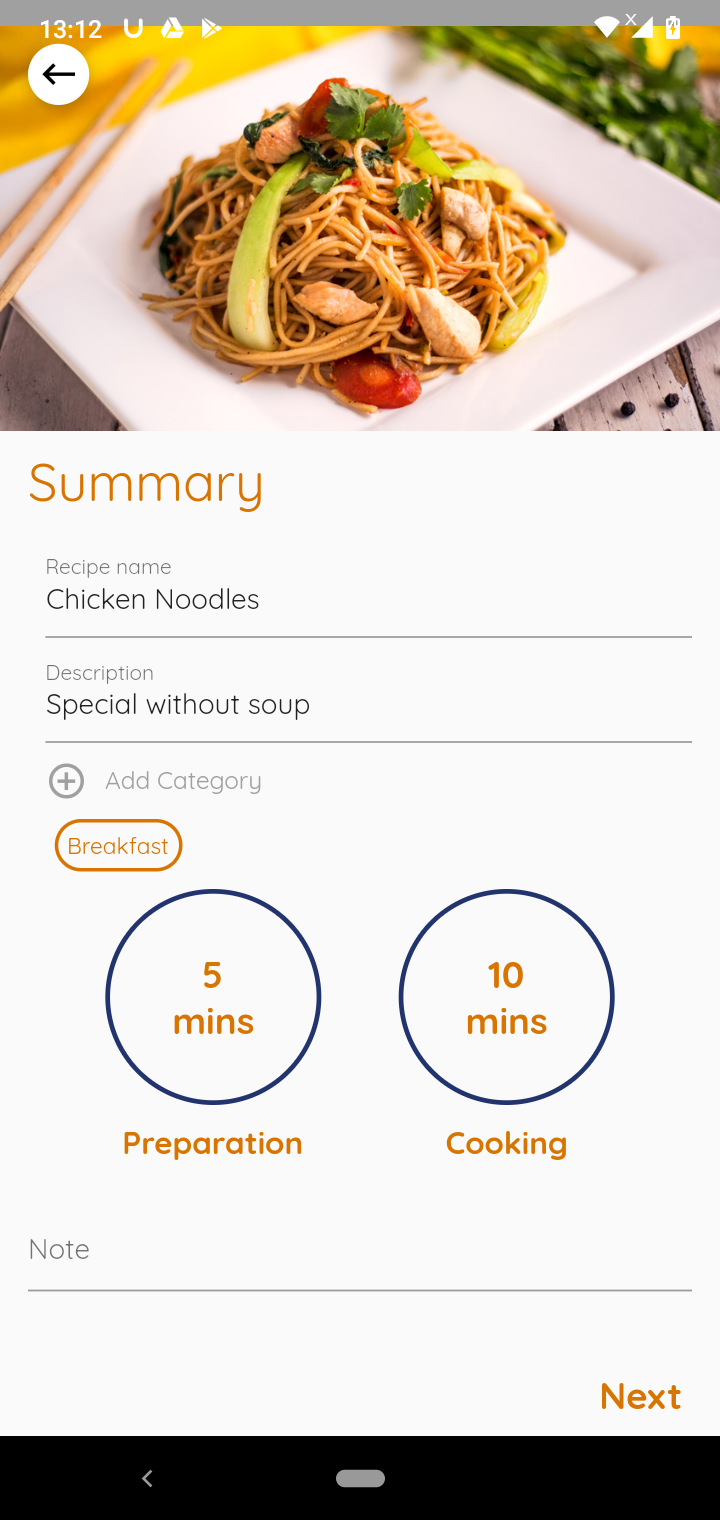
\includegraphics[scale=0.1]{Images/firednod_order.jpg}
    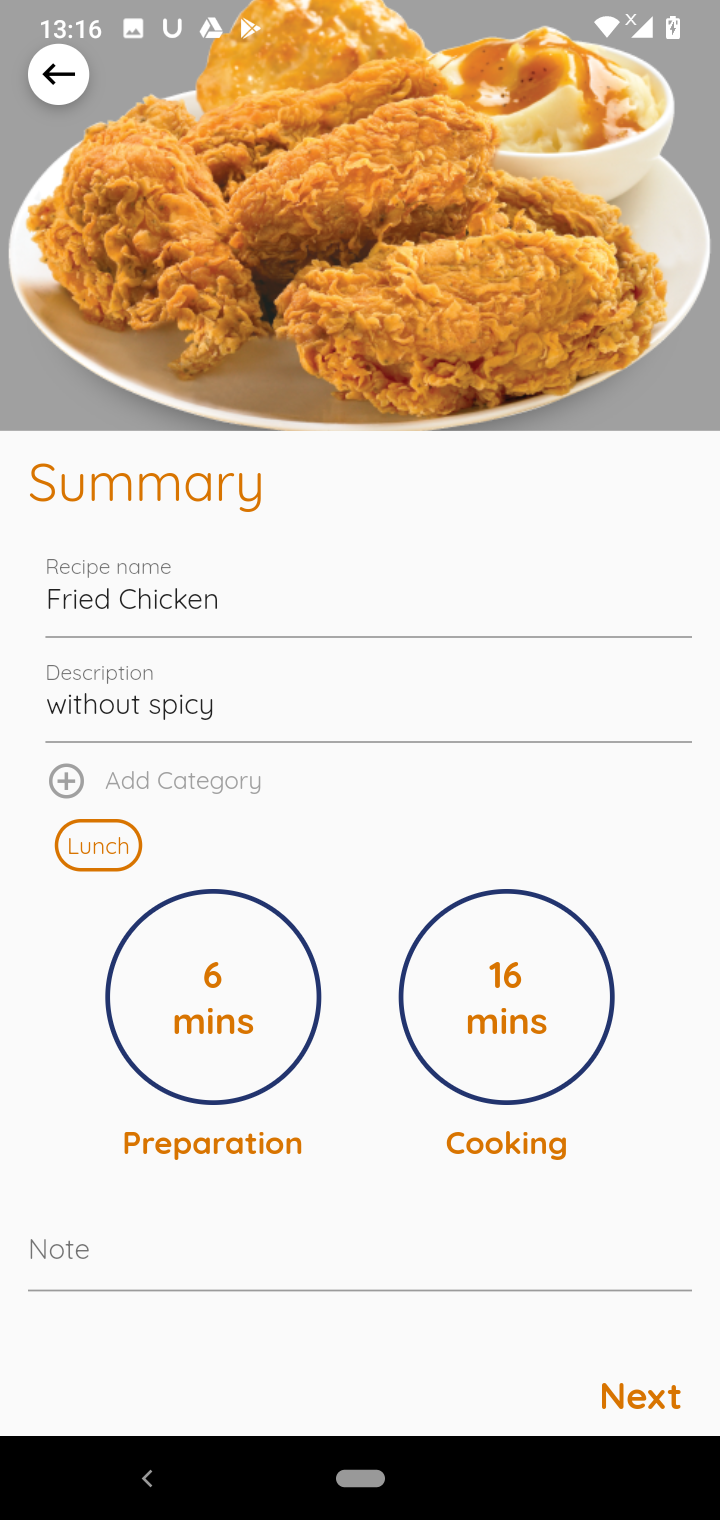
\includegraphics[scale=0.1]{Images/friechicken_order.jpg}
    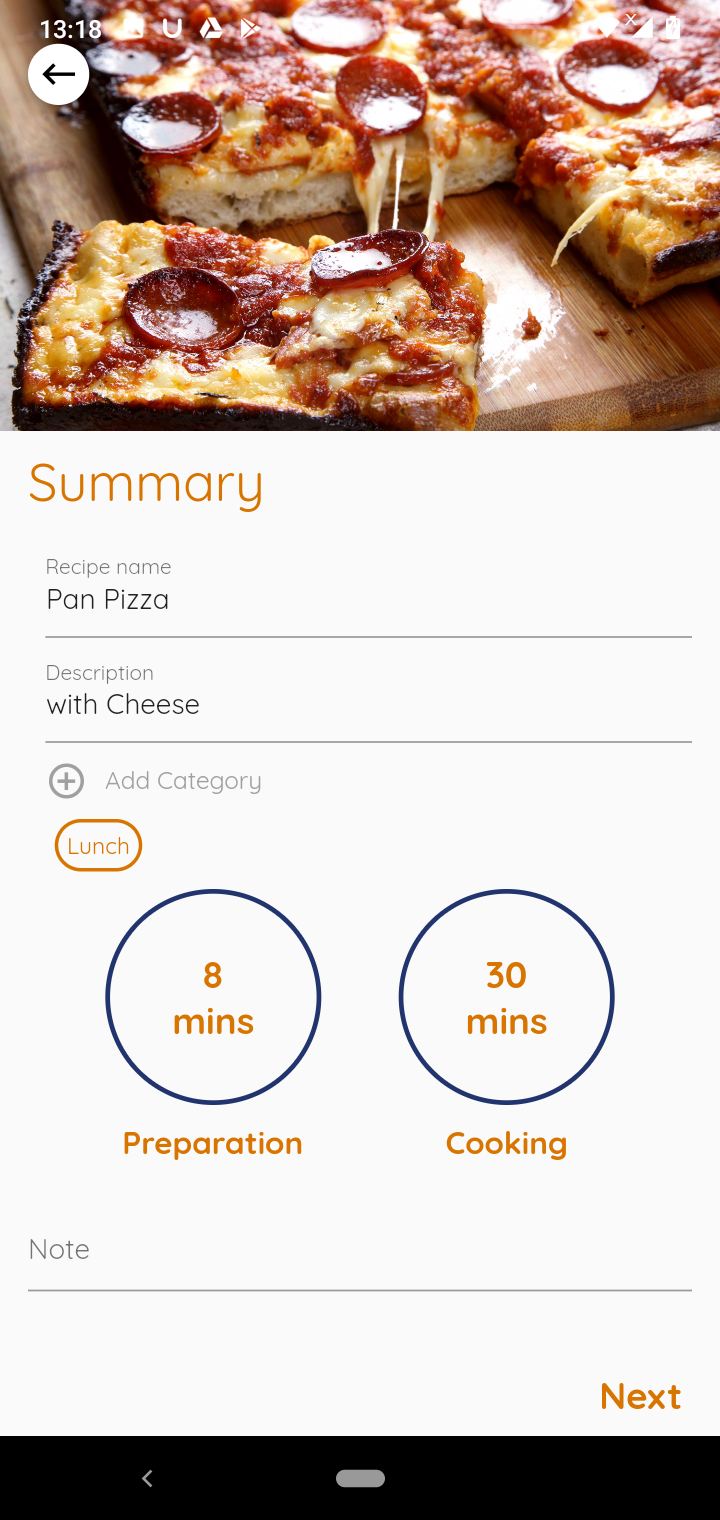
\includegraphics[scale=0.1]{Images/Panpizza_order.jpg}
    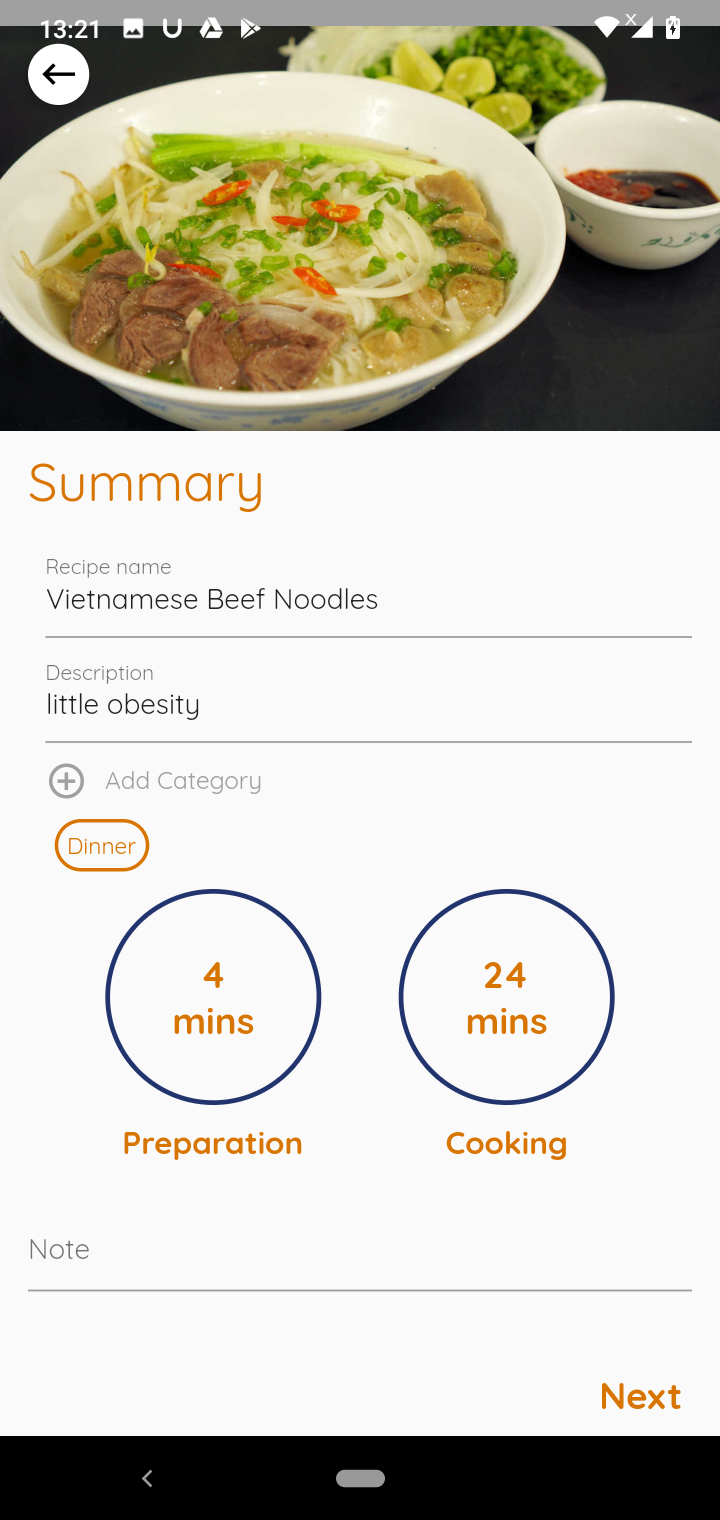
\includegraphics[scale=0.1]{Images/pho_order.jpg}
    \caption{Result for create new recipe success}
    For this step, a user can add Fired Noodles, Fried Chicken, Pan Pizza, and Vietnamese Beef Noodles. This activity is created to add the recipe include ingredient and direction steps.This stage will help the user can add photo of food and write Recipe name, ,Description, Add Category, Preparation or Cooking.After full filling, the next button will move to Ingredients and Direction when the user selects. 
    \label{fig:cookingbook}
    \end{figure}
    \newpage 
    
    
     -\textbf{Test case search recipe }: \\
    -Description : Test function when user search a recipe . \\
    ++ Step 1 : Open the app  \\
    ++ Step 2 : Go to Search tab \\
    ++ Step 3 : Fill keyword into search box  \\
    ++ Step 4 : Click search button  \\
    -Expected result : The list recipe should show correct with keyword filled-in . \\
    -Actual Result : As expected \\
    -Pass/Fail : Passed \\
    -Comment :  \\
    -Result : 
    \begin{figure}[h!]
    \centering
    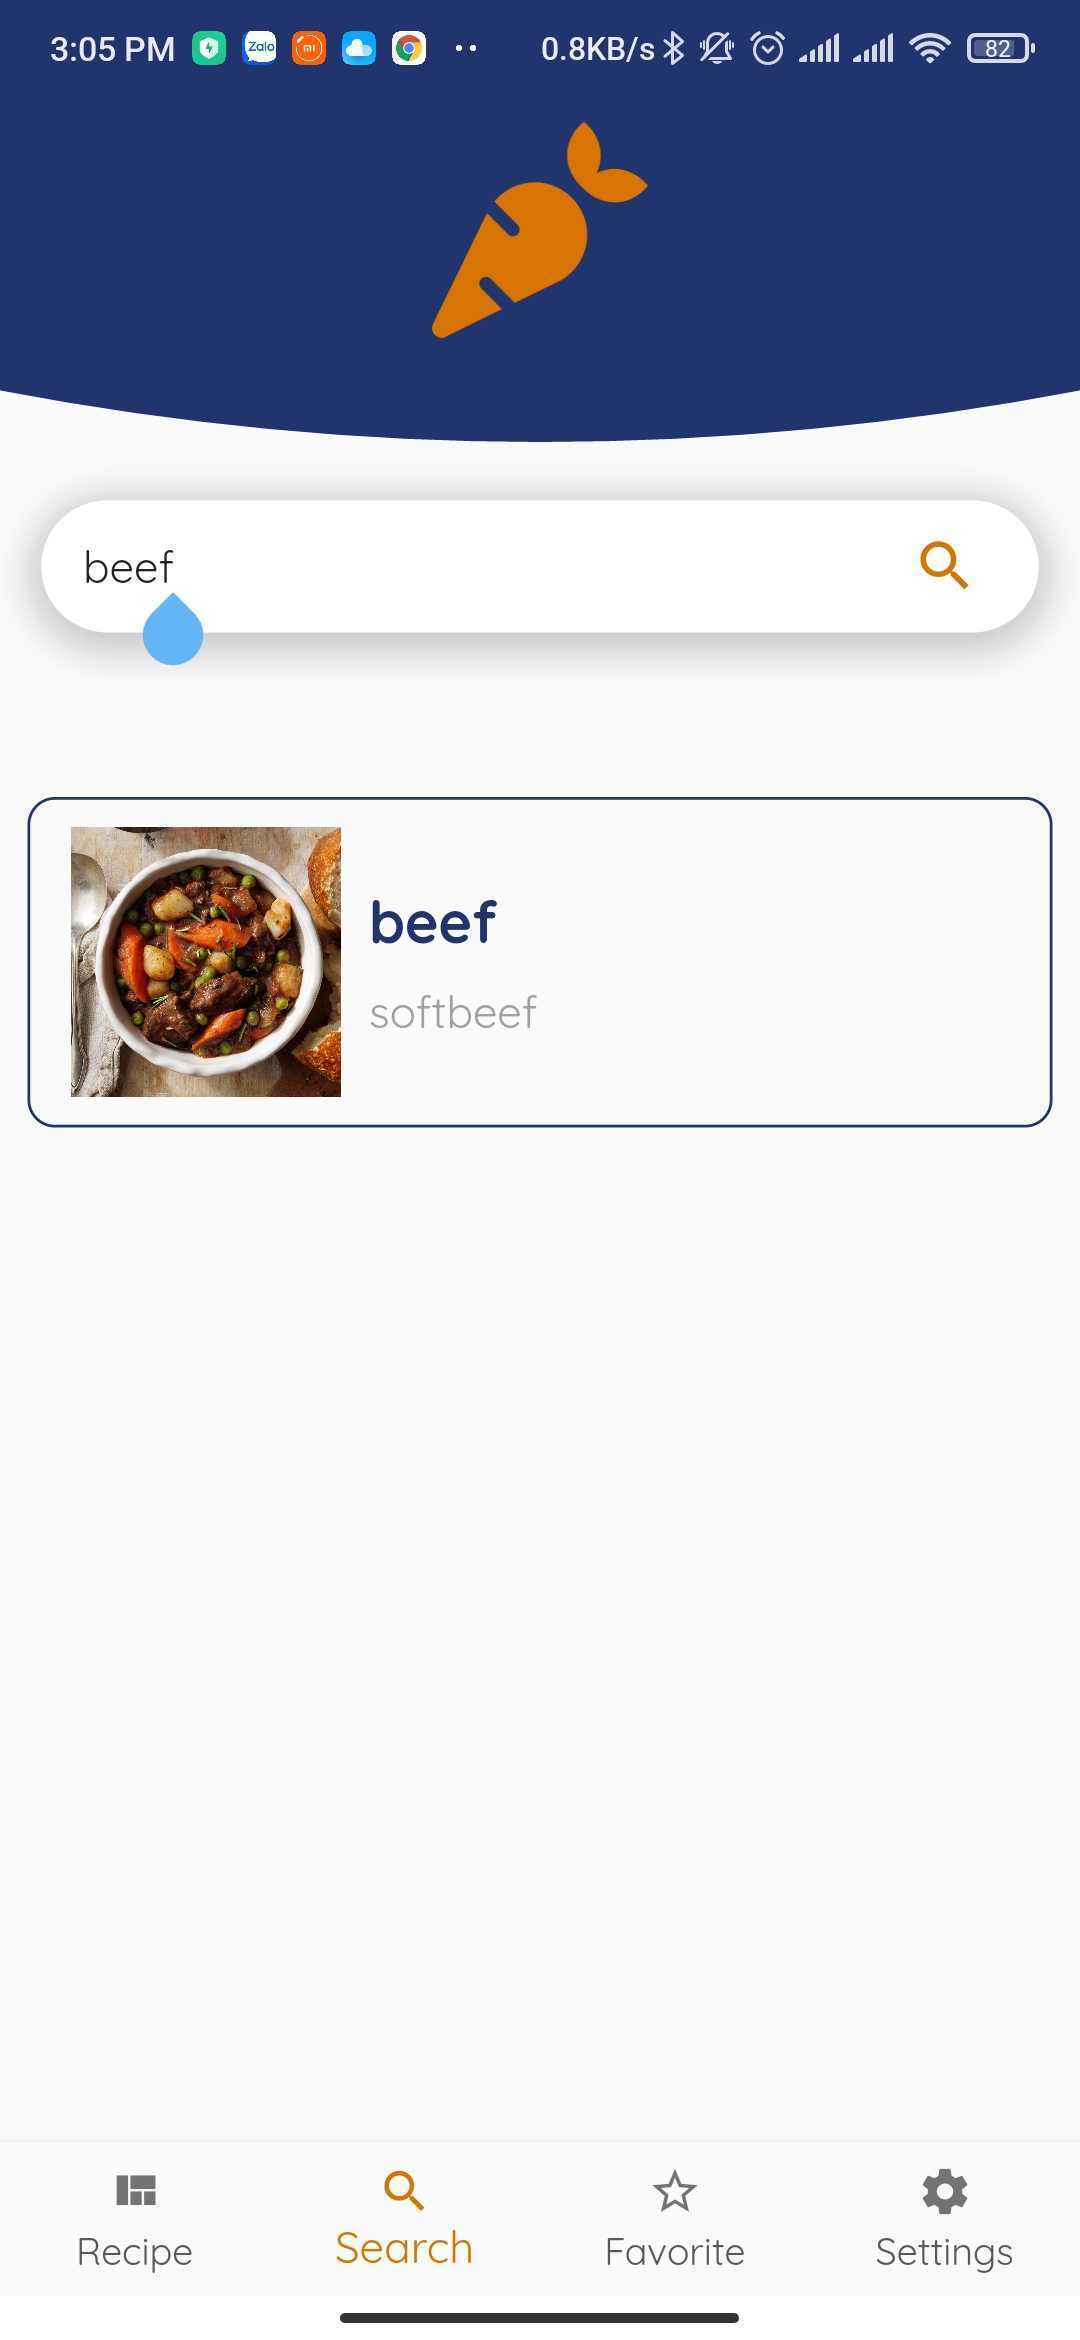
\includegraphics[scale=0.15]{Images/search1.jpg}
    
    \caption{Result for search 'beef' keyword}
    
    \label{fig:cookingbook}
    \end{figure}
    \newpage 
    
 -\textbf{Test case add category for recipe }: \\
    -Description : Test function when user view a recipe. \\
    ++ Step 1 : Open the app  \\
    ++ Step 2 : Go to Recipe Tab \\
    ++ Step 3 : Click (+) Button in  \\
    ++ Step 4 : Fill-in information of new recipe \\
    ++ Step 5 : Click add categories Button  \\
    ++ Step 6 : Select Category  \\
    ++ Step 7 : Click Save Button \\
    -Expected result : Category must show as same as when user create recipe. \\
    -Actual Result : As expected \\
    -Pass/Fail : Passed \\
    -Comment : 
    -Result:
    \begin{figure}[h!]
    \centering
    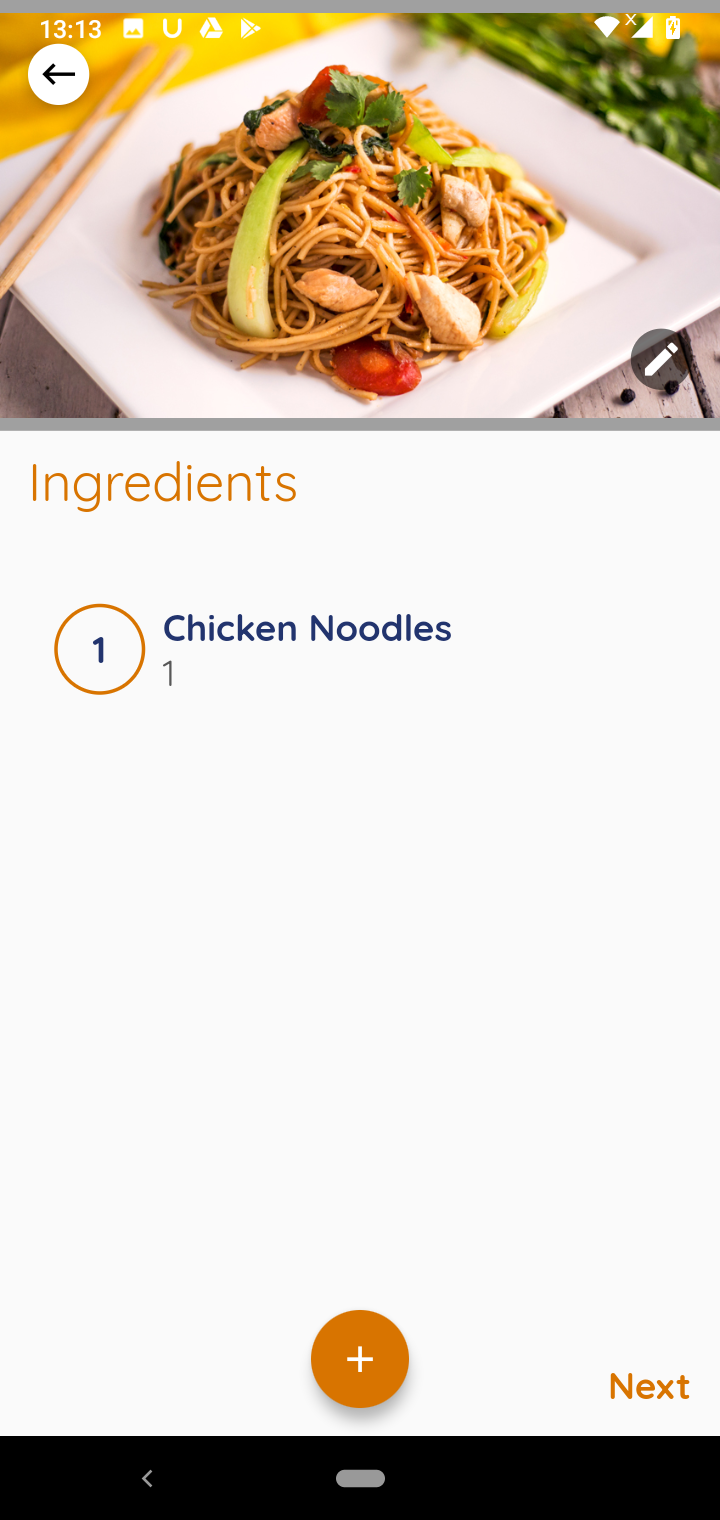
\includegraphics[scale=0.1]{Images/frienod_ingre.jpg}
    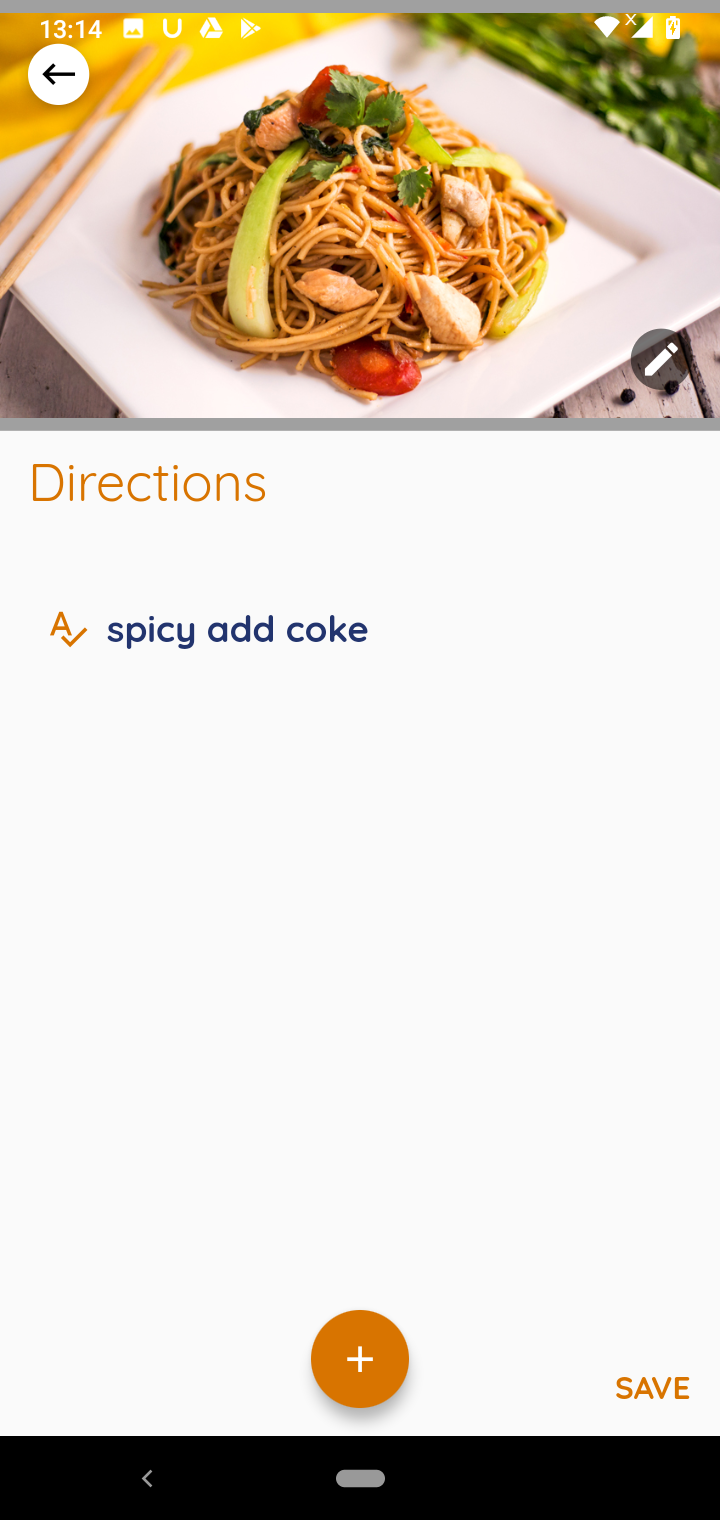
\includegraphics[scale=0.1]{Images/frienod_dire.jpg}
    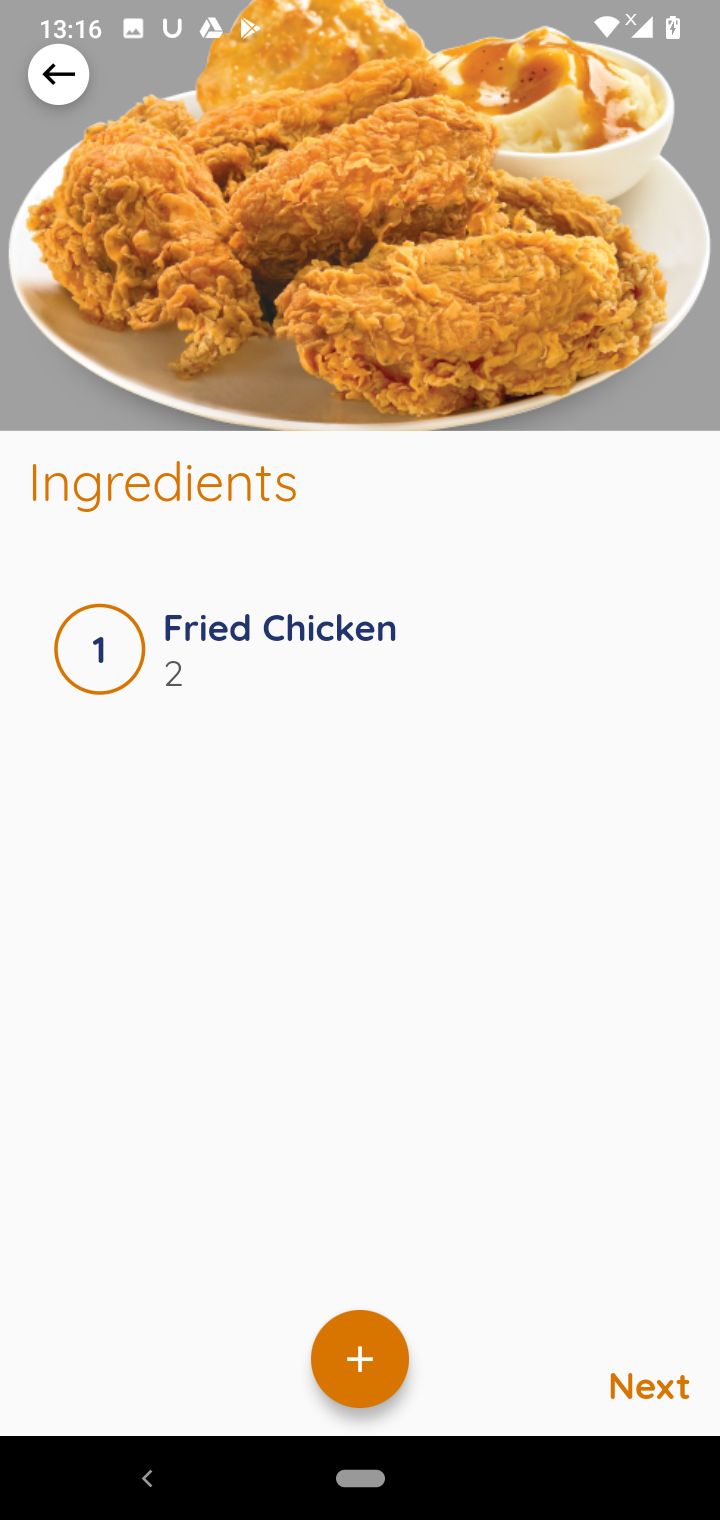
\includegraphics[scale=0.1]{Images/friechick_ingre.jpg}
    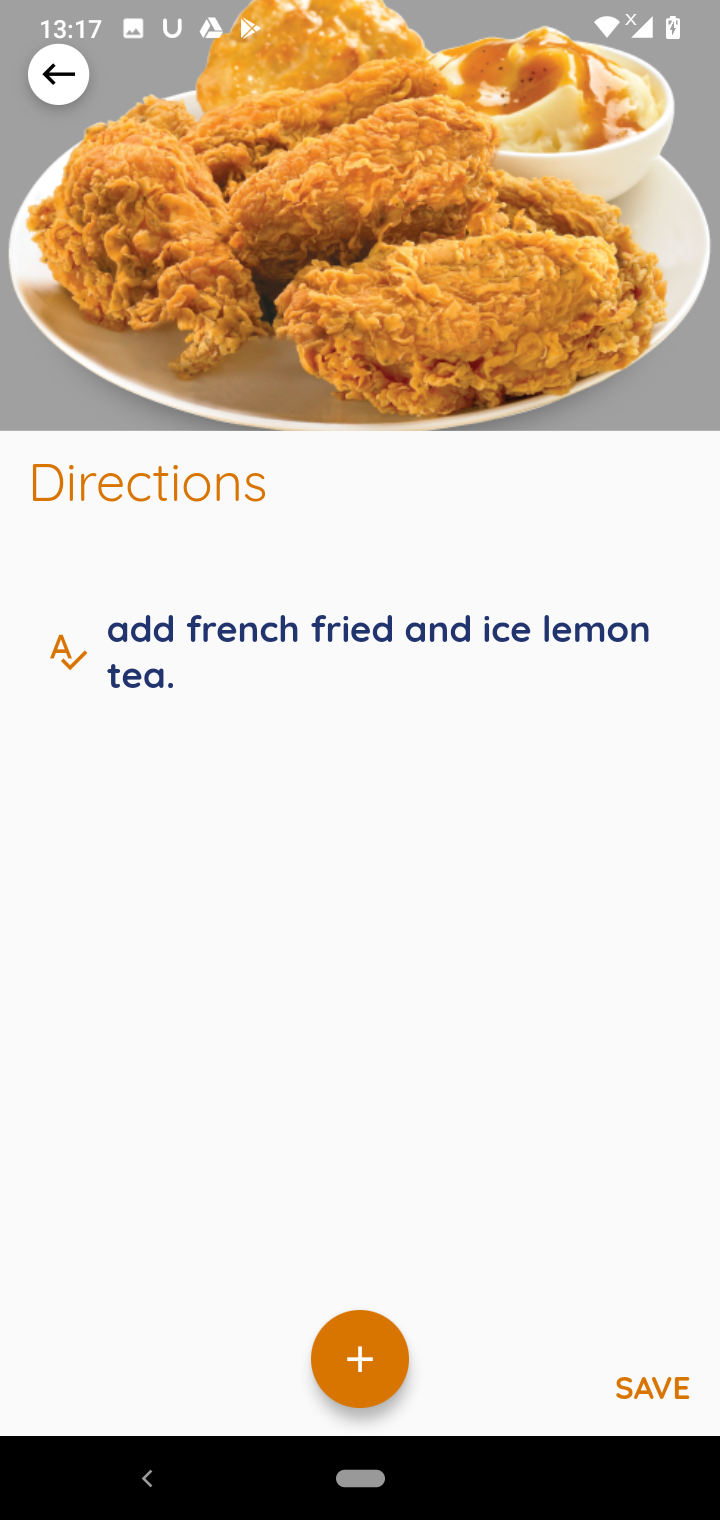
\includegraphics[scale=0.1]{Images/firechick_direc.jpg}
    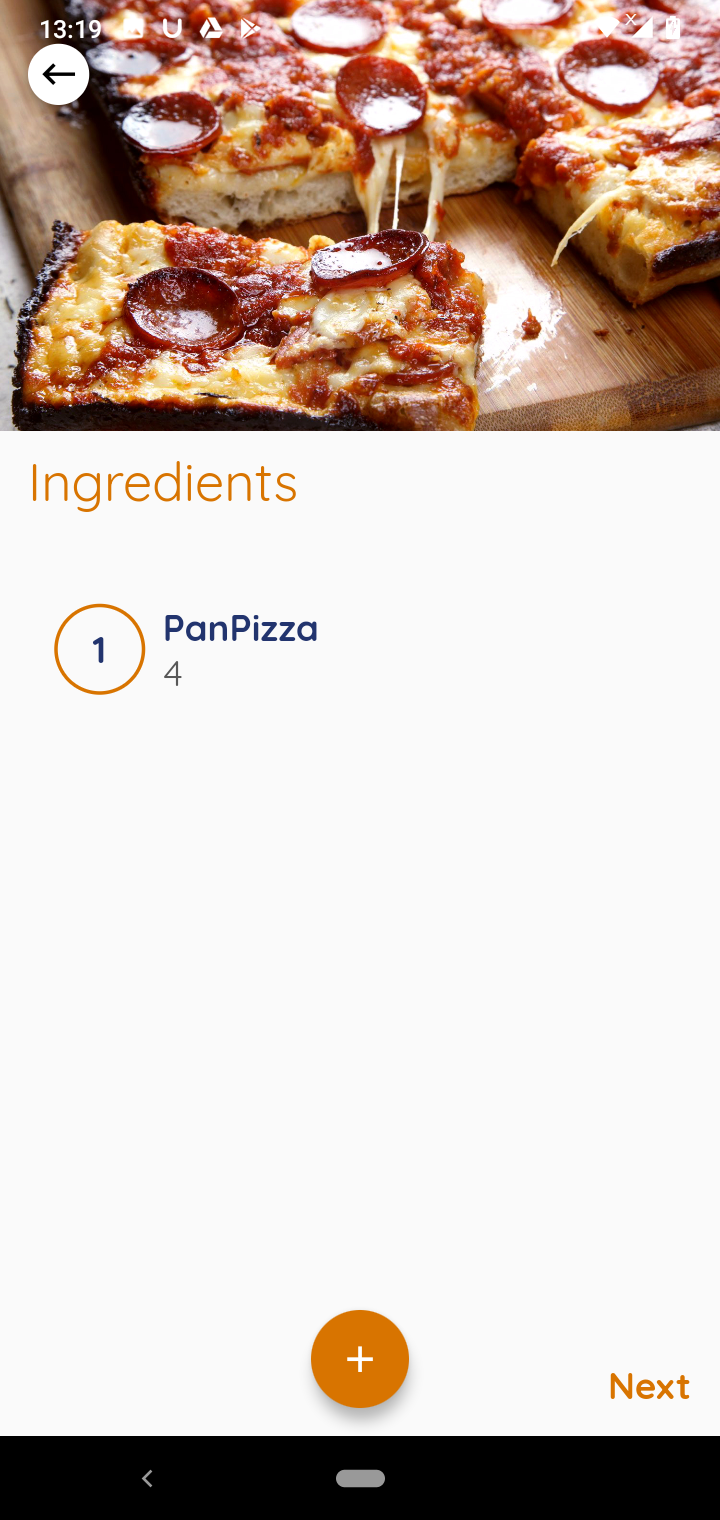
\includegraphics[scale=0.1]{Images/Panpizza_ingre.jpg}
    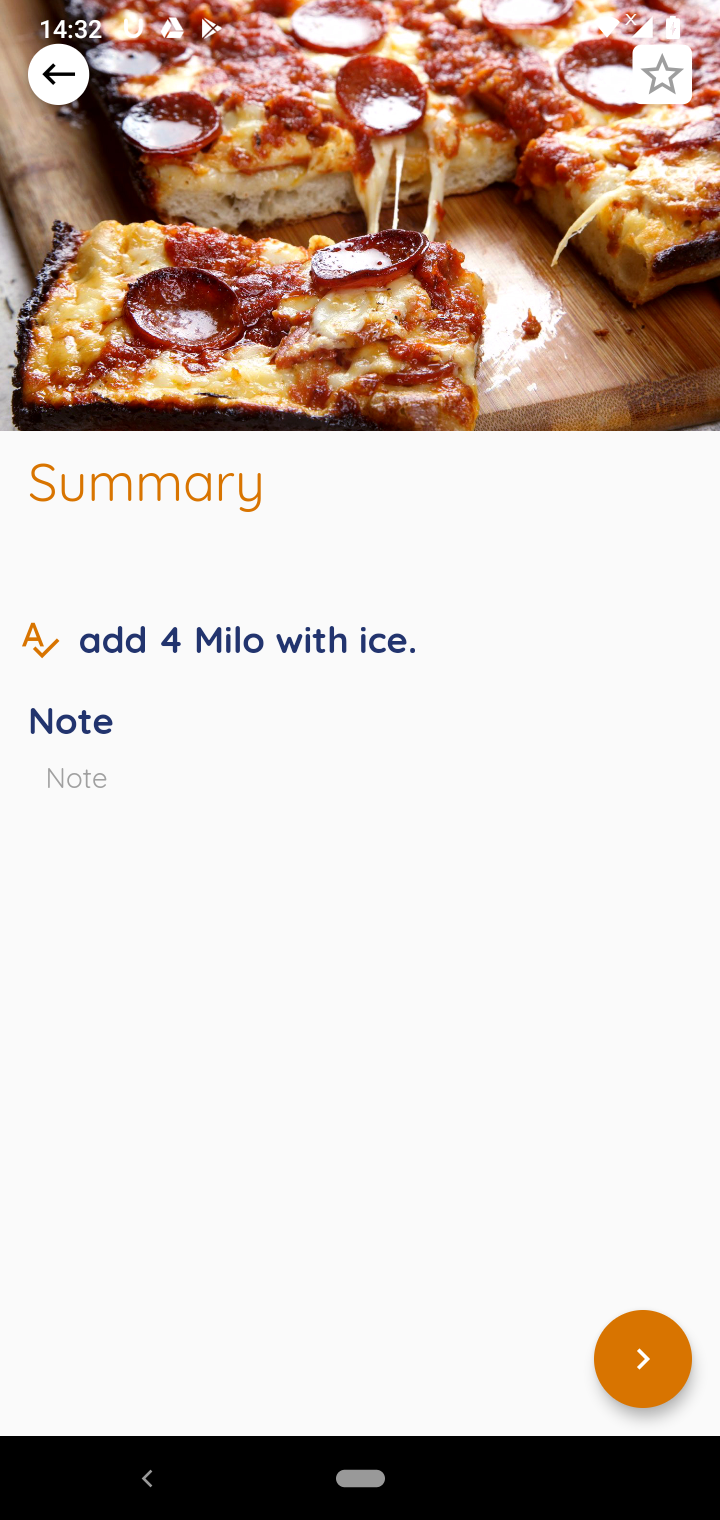
\includegraphics[scale=0.1]{Images/Panpizza_dire.jpg}
    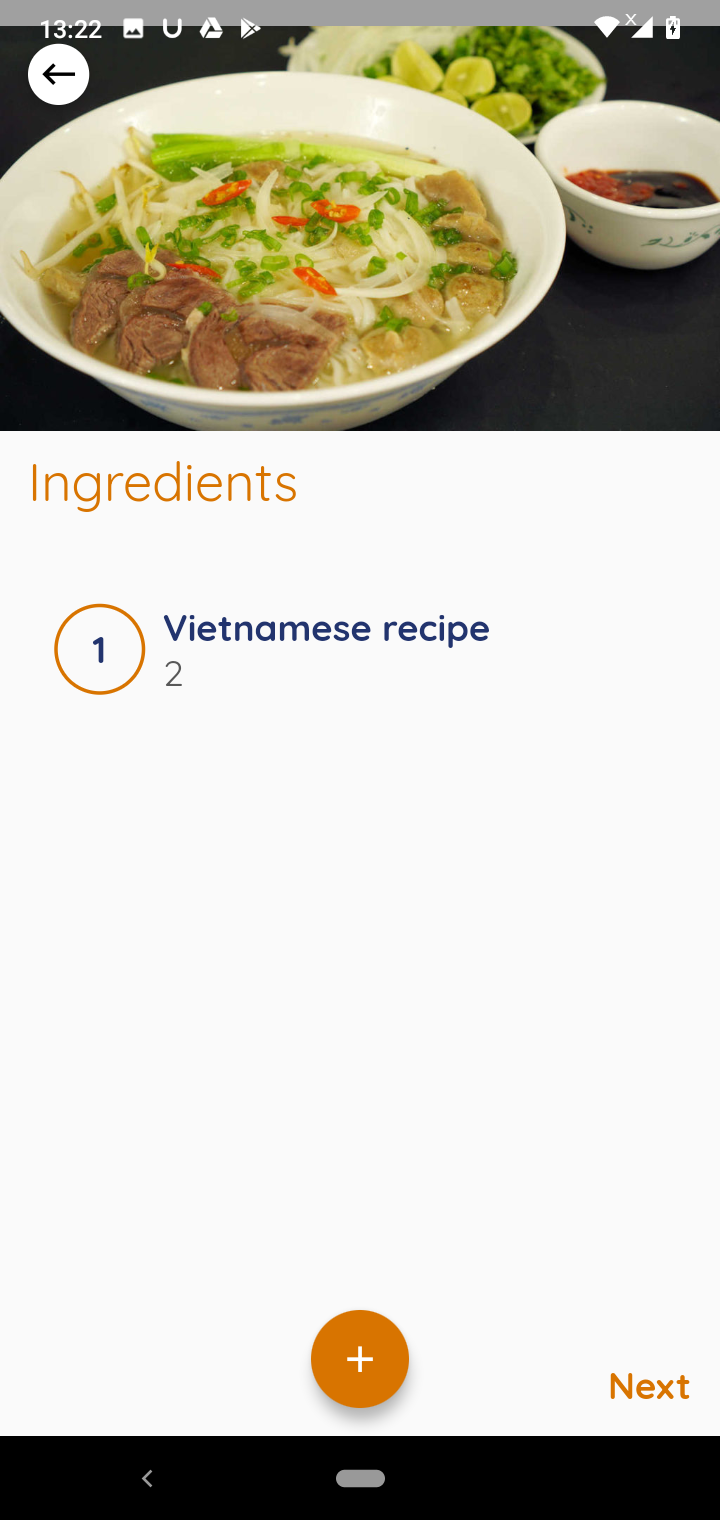
\includegraphics[scale=0.1]{Images/pho_ingre.jpg}
    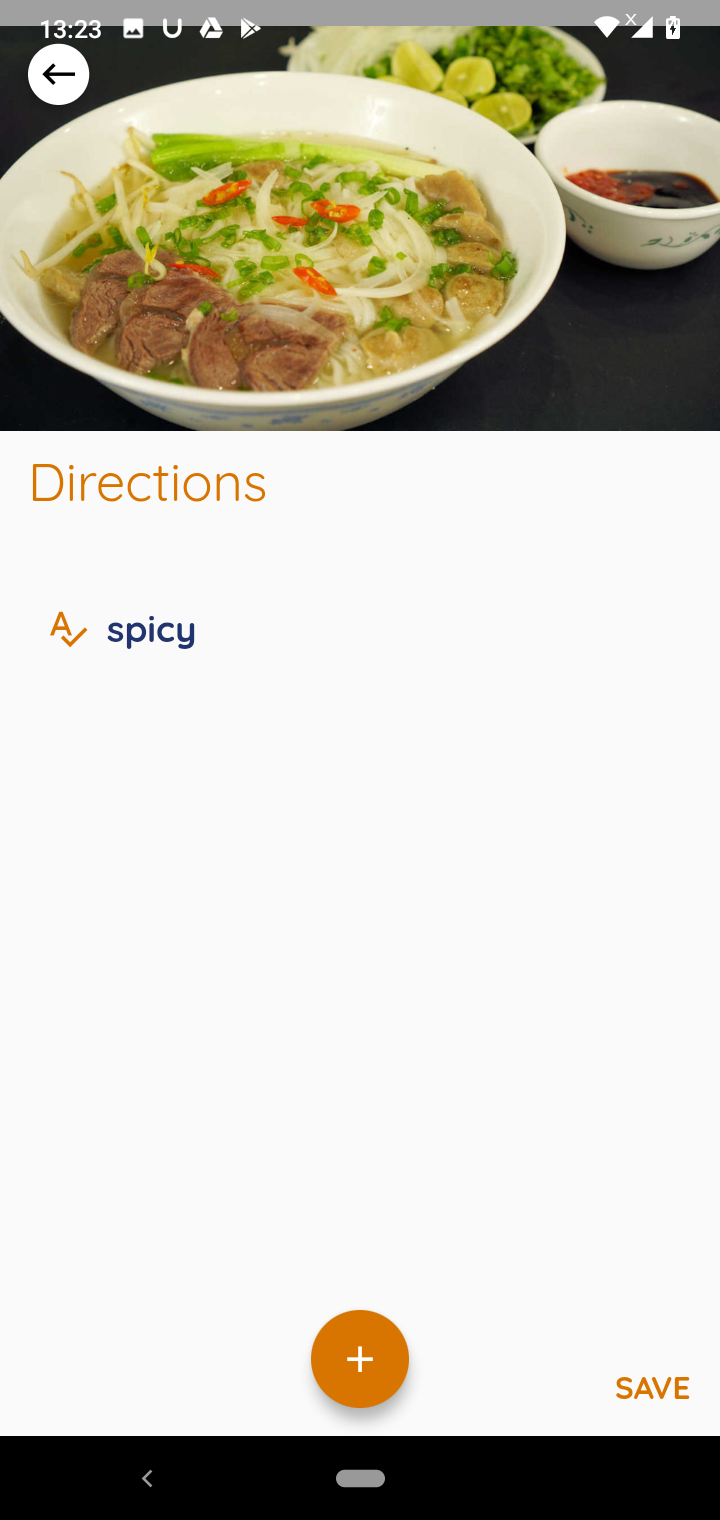
\includegraphics[scale=0.1]{Images/pho_dire.jpg}
    The categories include Fired Noodles, Fired Chicken, Pan Pizza, and Vietnamese Beef Food.Besides the user can be able to add drinks. In addition, the user can view the time for Preparation or Cooking. 
    \caption{Result for create new recipe success}
    \label{fig:cookingbook}
    \end{figure}
\newpage 
-\textbf{Test case add recipe to favorite }: \\
    -Description : Test function when user add a recipe to their list of favorite . \\
    ++ Step 1 : Open the app  \\
    ++ Step 2 : Go to Recipe Tab \\
    ++ Step 3 : Select a recipe to view detail   \\
    ++ Step 4 : Click star Button in the top of right corner to add an item to favorite list\\
    ++ Step 5 : Go back into main screen  \\
    ++ Step 6 :  Go to tab Favorite  \\
    ++ Step 7 : Check if favorite recipe just added into the list \\
    -Expected result : When added into favorite list, and open the tab Favorite, it should appear the icon just added. . \\
    -Actual Result : As expected \\
    -Pass/Fail : Passed \\
    -Comment : 
    -Result:
    \begin{figure}[h!]
    \centering
    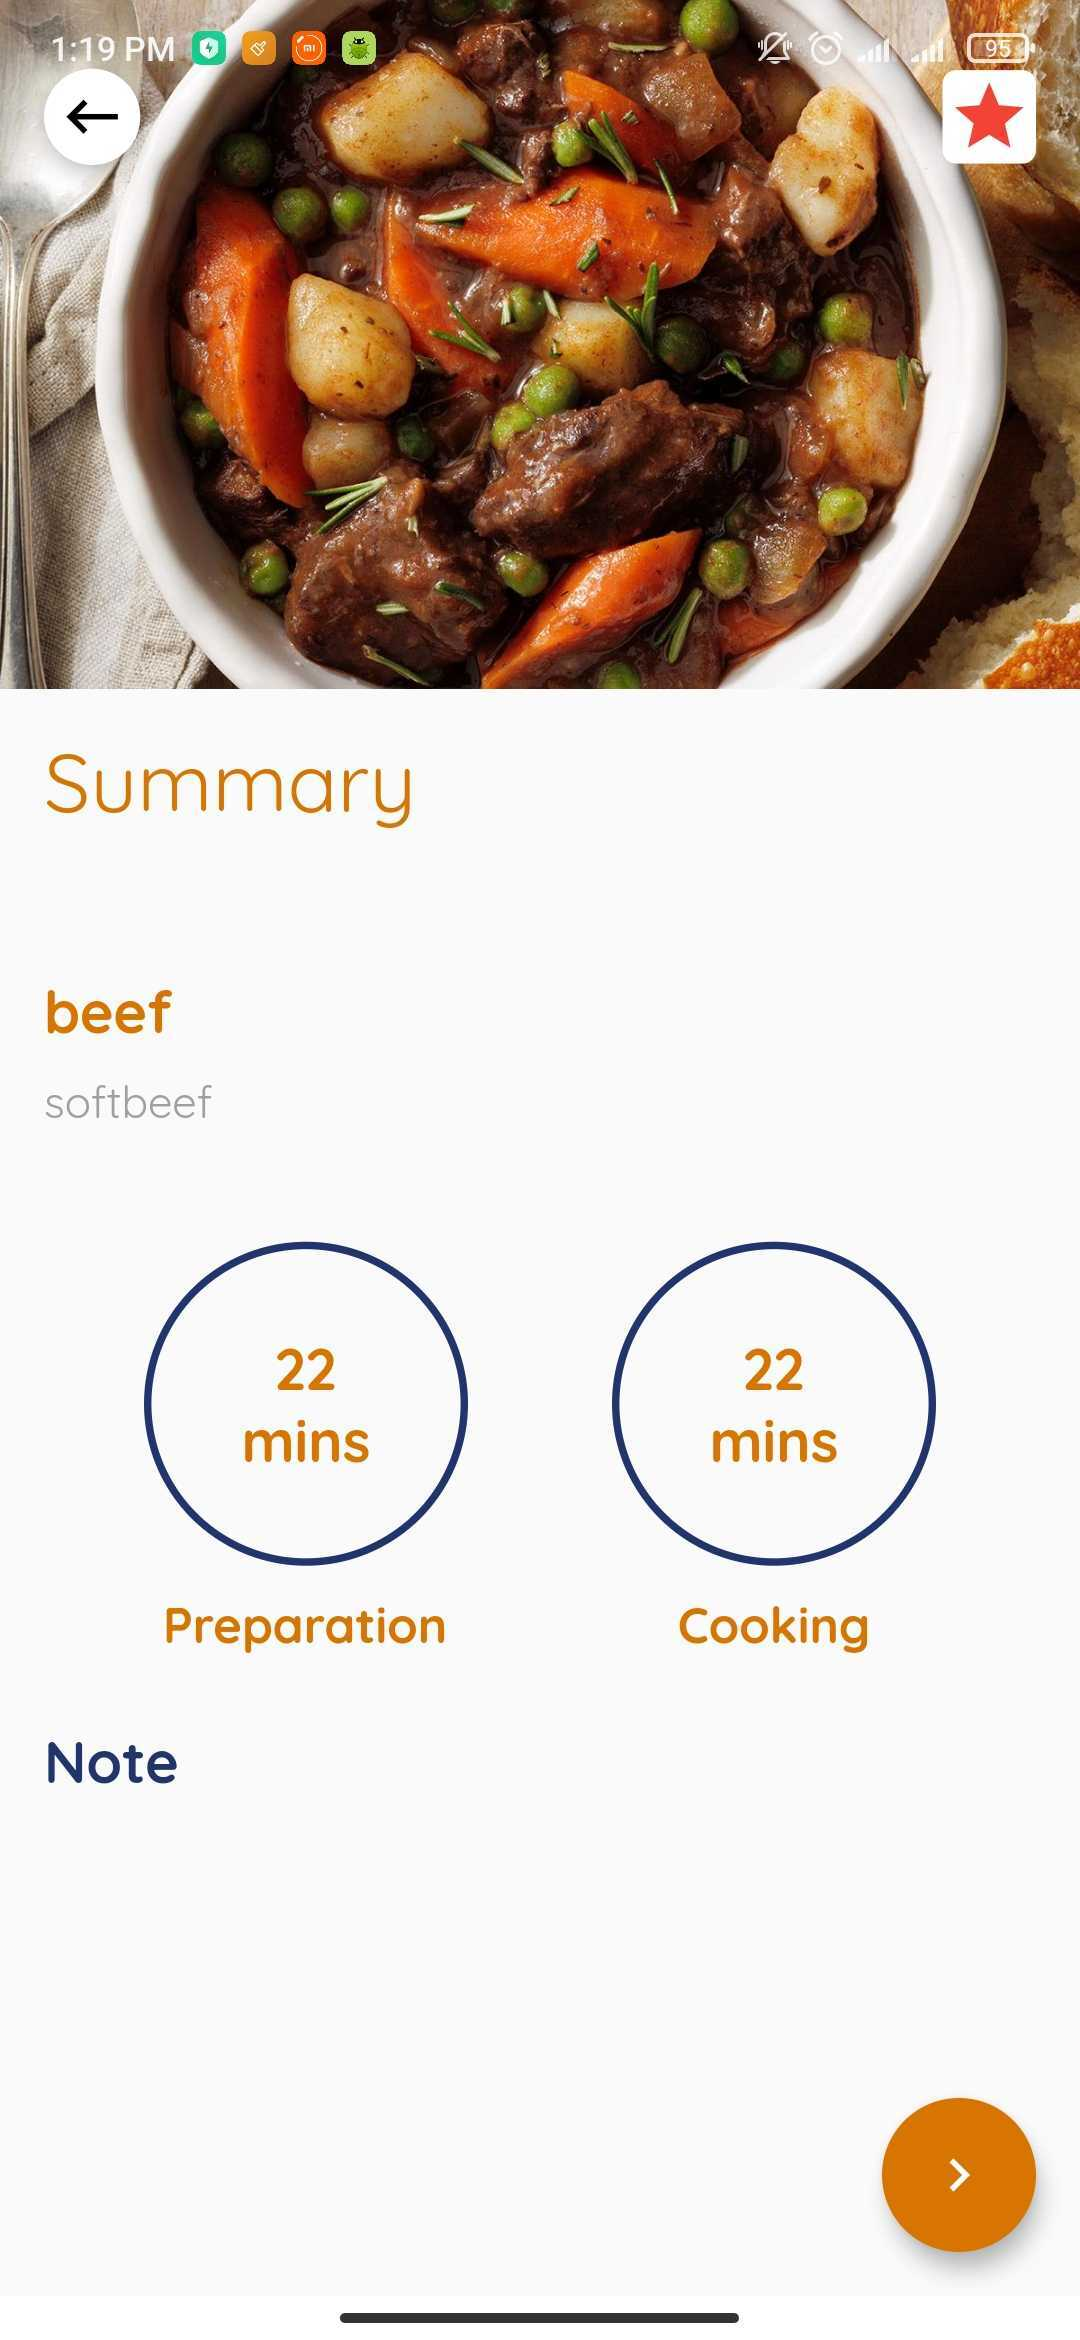
\includegraphics[scale=0.1]{Images/AddToFavorite.jpg}
    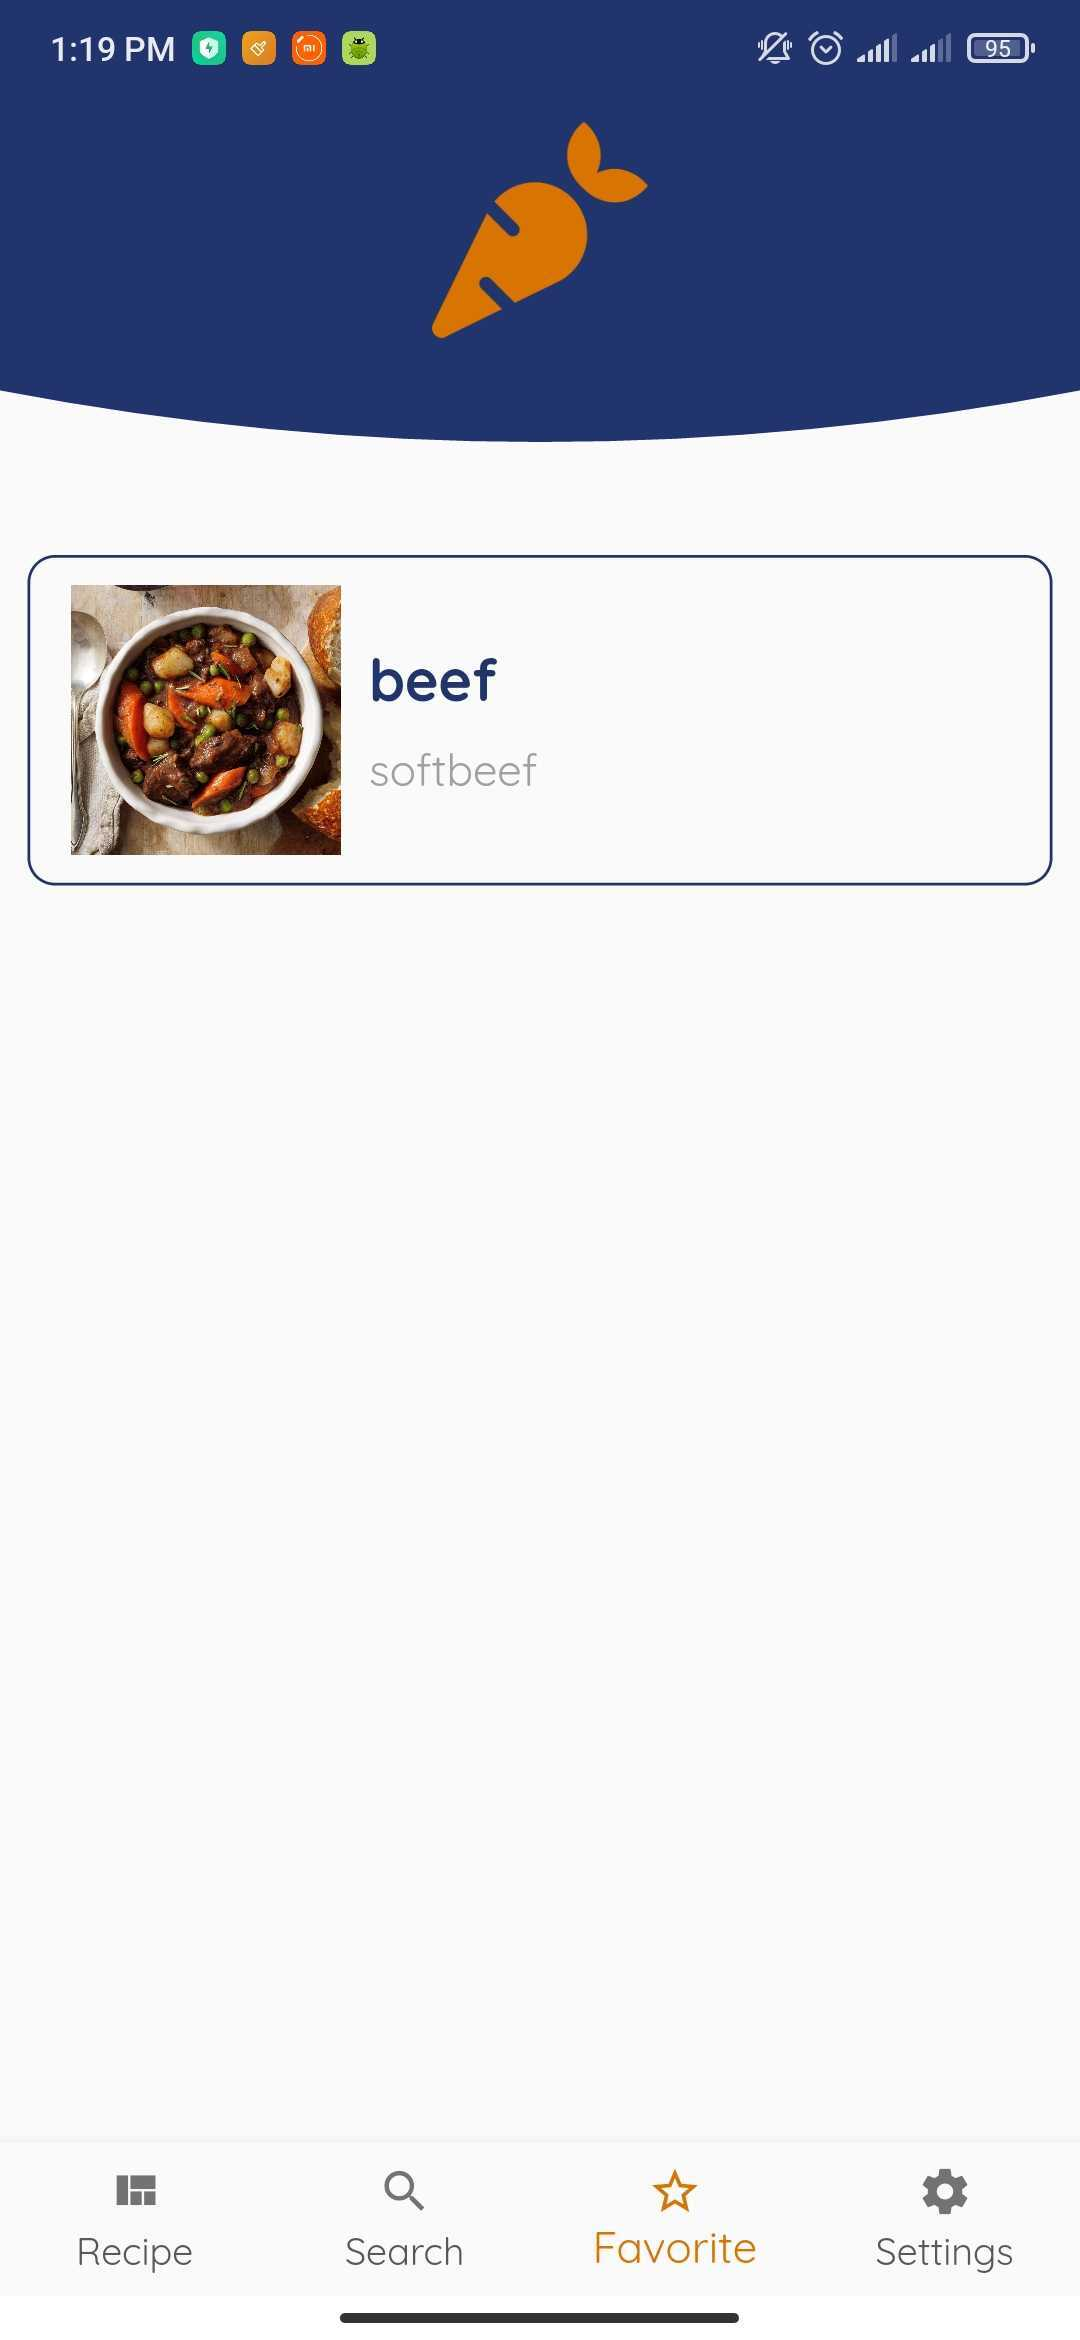
\includegraphics[scale=0.1]{Images/FavoriteList.jpg}
    \caption{test for add to favorite}
    \label{fig:cookingbook}
    \end{figure}
\newpage 
 -\textbf{Test case remove recipe to favorite }: \\
    -Description : Test function when user remove a recipe to their list of favorite . \\
    ++ Step 1 : Open the app  \\
    ++ Step 2 : Go to Recipe Tab \\
    ++ Step 3 : Select a recipe to view detail   \\
    ++ Step 4 : Un-check star Button in the top of right corner to add an item to favorite list\\
    ++ Step 5 : Go back into main screen  \\
    ++ Step 6 :  Go to tab Favorite  \\
    ++ Step 7 : Check if favorite recipe just remove into the list \\
    -Expected result : When remove a recipe into favorite list, and open the tab Favorite, it should not appear the recipe in favorite list. If the list empty, it should show message as this favorite list is empty.
    -Actual Result : As expected \\
    -Pass/Fail : Passed \\
    -Comment : 
    -Result:
    \begin{figure}[h!]
    \centering
    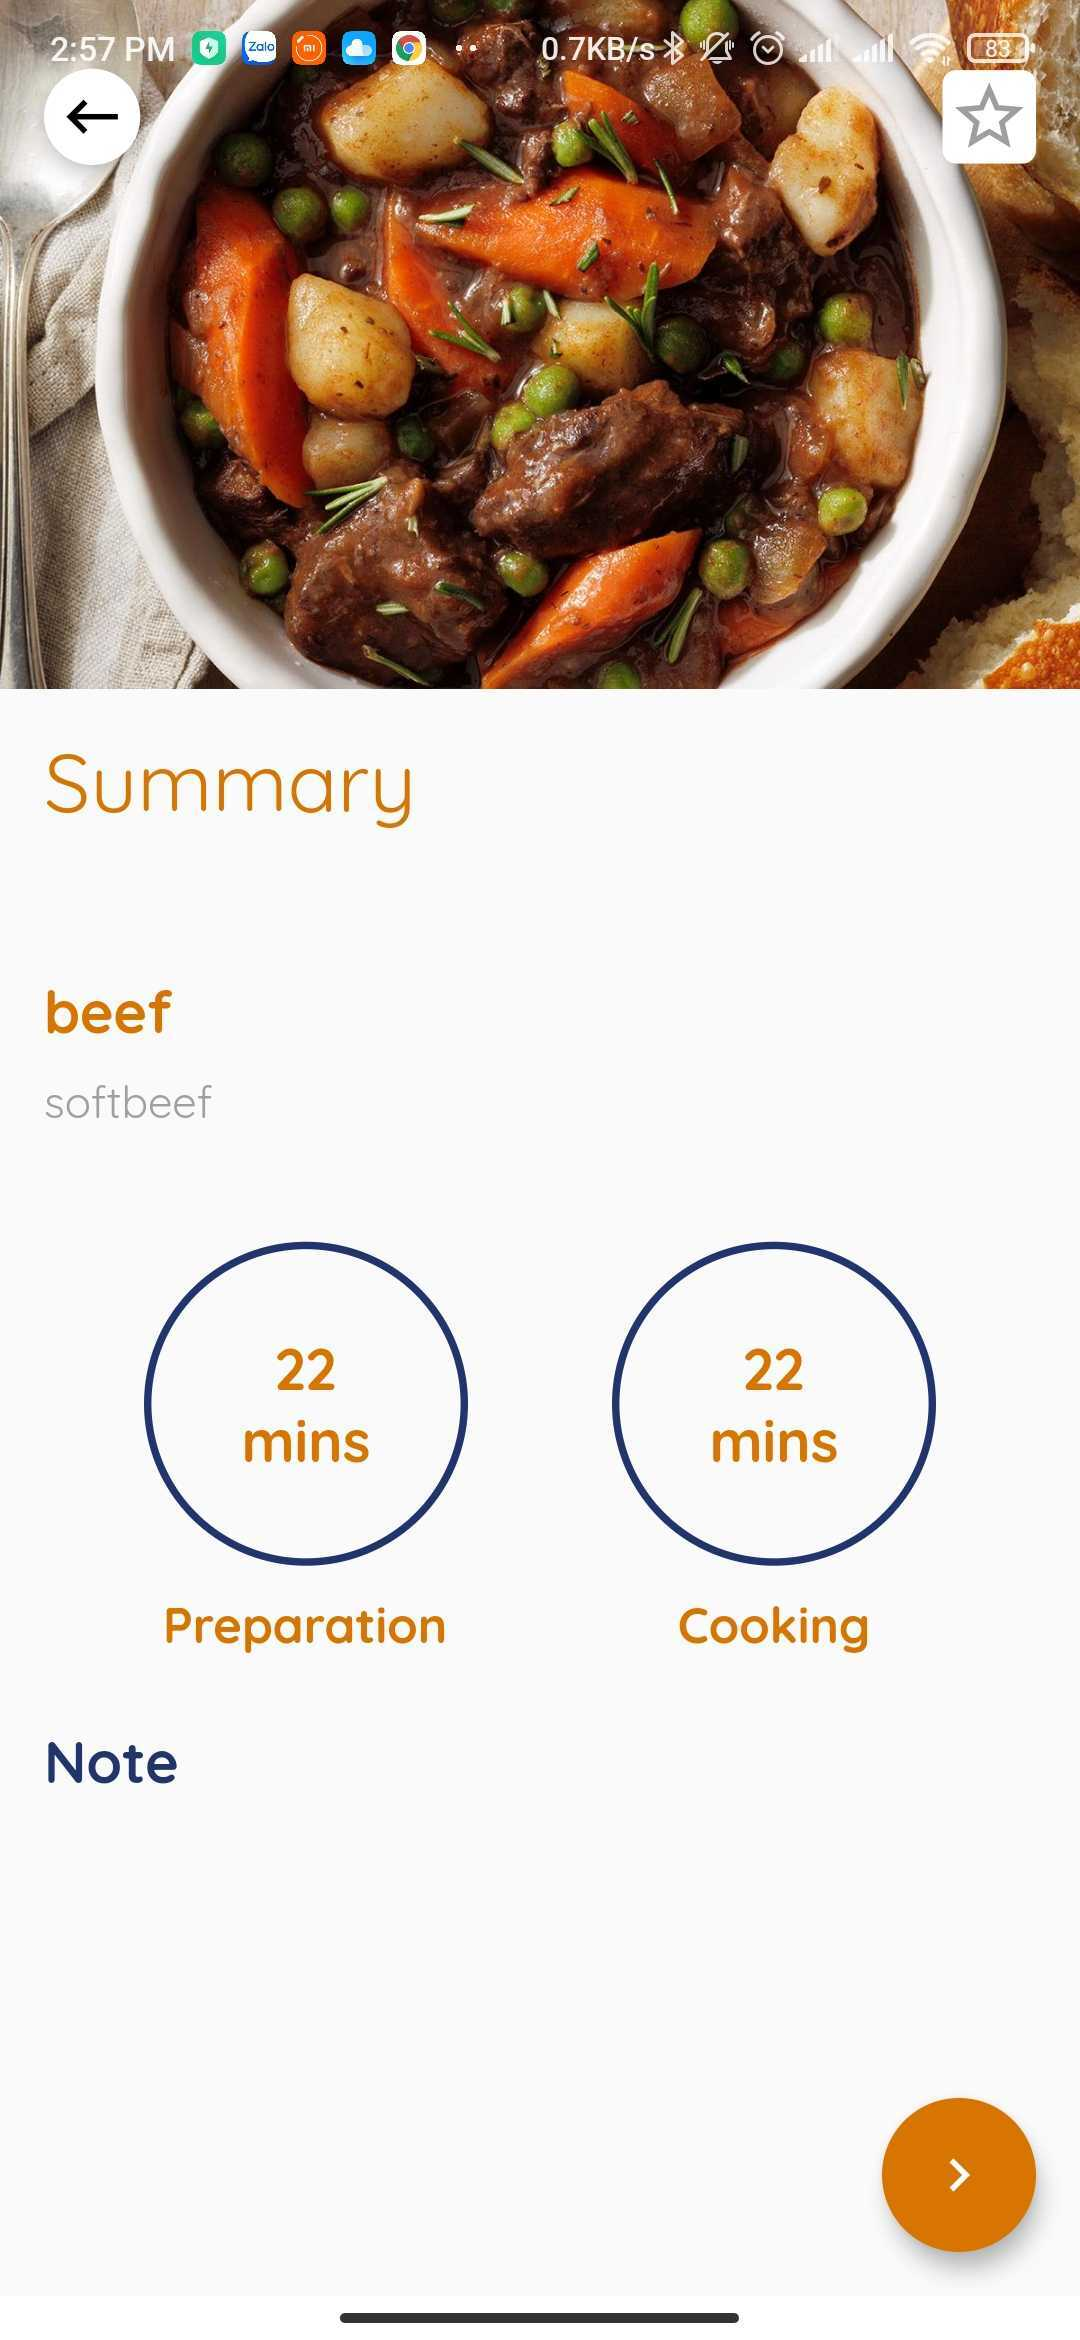
\includegraphics[scale=0.1]{Images/Favorite-unchecked.jpg}
    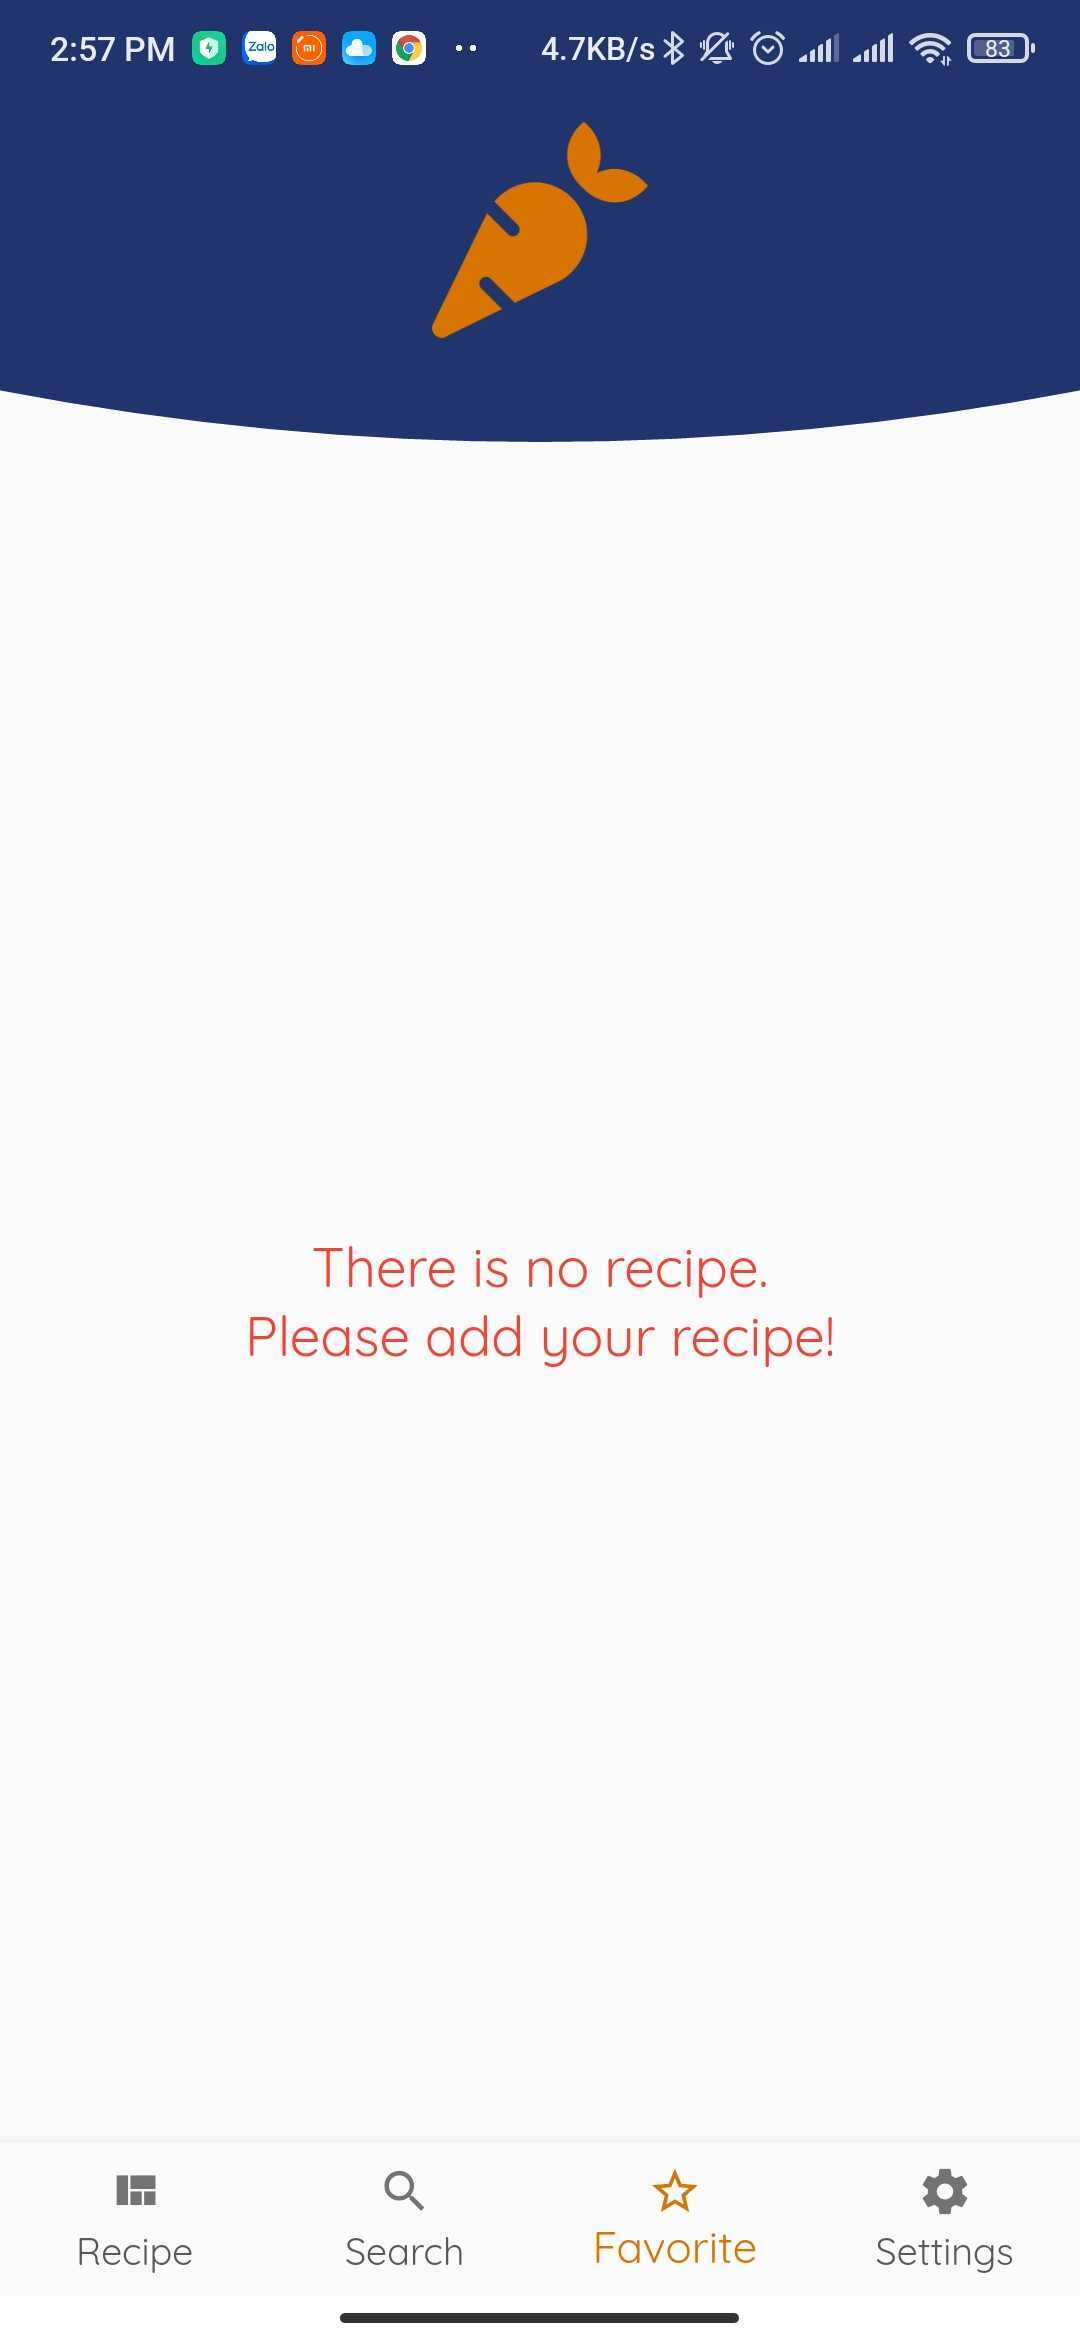
\includegraphics[scale=0.1]{Images/Favorite-emptylist.jpg}
    \caption{test for remove to favorite}
    \label{fig:cookingbook}
    \end{figure}
\newpage 
    -\textbf{Test go-to setting screens }: \\
    -Description : Test function when user goto setting screen. \\
    ++ Step 1 : Open the app  \\
    ++ Step 2 : Go to Settings tab \\
    -Expected result : It should show setting pages include 4 buttons : Share, Help, Language, About button. \\
    -Actual Result : As expected \\
    -Pass/Fail : Passed \\
    -Comment :  \\
    -Result : 
    \begin{figure}[h!]
    \centering
    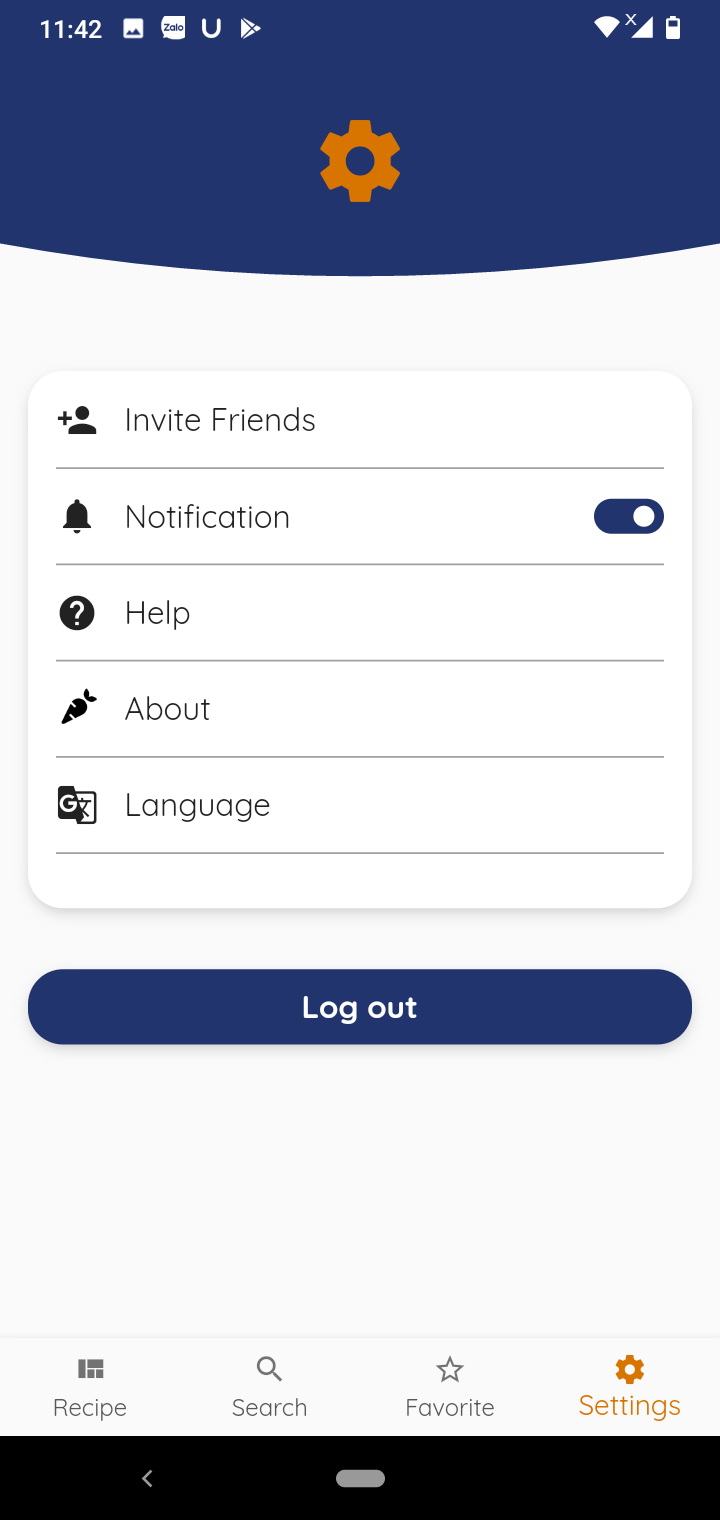
\includegraphics[scale=0.20]{Images/Settings.jpg}
    \caption{Result for go-to setting tabs}
    For this function, it will display the layout with some functions like Share, Help, Language, and About.
    \label{fig:cookingbook}
    \end{figure}
 \newpage
\subsubsection{WHITE BOX TEST} 
\textbf{Unit test}: \\
        Built-in test package of Flutter (https://flutter.dev/docs/cookbook/testing/unit/introduction) \\
        “Mock”: use mockito (https://flutter.dev/docs/cookbook/testing/unit/mocking) \\
        CI (continuous integration): Github action \\
        When we merge code from any branch to “master” branch, pre-define script on Github action will be triggered to run all the tests. If the tests are passed, it continues to build .apk file and stores it on Github (we probably send this apk to Slack channel if we need).
        State management in Flutter: We use mobX (https://mobx.netlify.com) because of its simplicity.\\ \\
    Two main business logic repository need to test is :  \\
    \textbf{Unit test for recipe repository}: 
    \begin{enumerate}
        \item Test create recipe \textbf{(Passed)}
        \item Test get recipes \textbf{(Passed)}
        \item Test get recipe by category id \textbf{(Passed)}
        \item Test get favorite recipes \textbf{(Passed)}
        \item Test search recipes \textbf{(Passed)}
        \item Test add recipe to favorite \textbf{(Passed)}
    \end{enumerate} 
    \newline
\textbf{Unit test for categories repository}: 
      \begin{enumerate}
        \item Test create category \textbf{(Passed)}
        \item Test update category \textbf{(Passed)}
        \item Test get categories \textbf{(Passed)}
    \end{enumerate} 
    \newpage
    Unit test for categories : 
    \begin{figure}[h!]
            \centering
            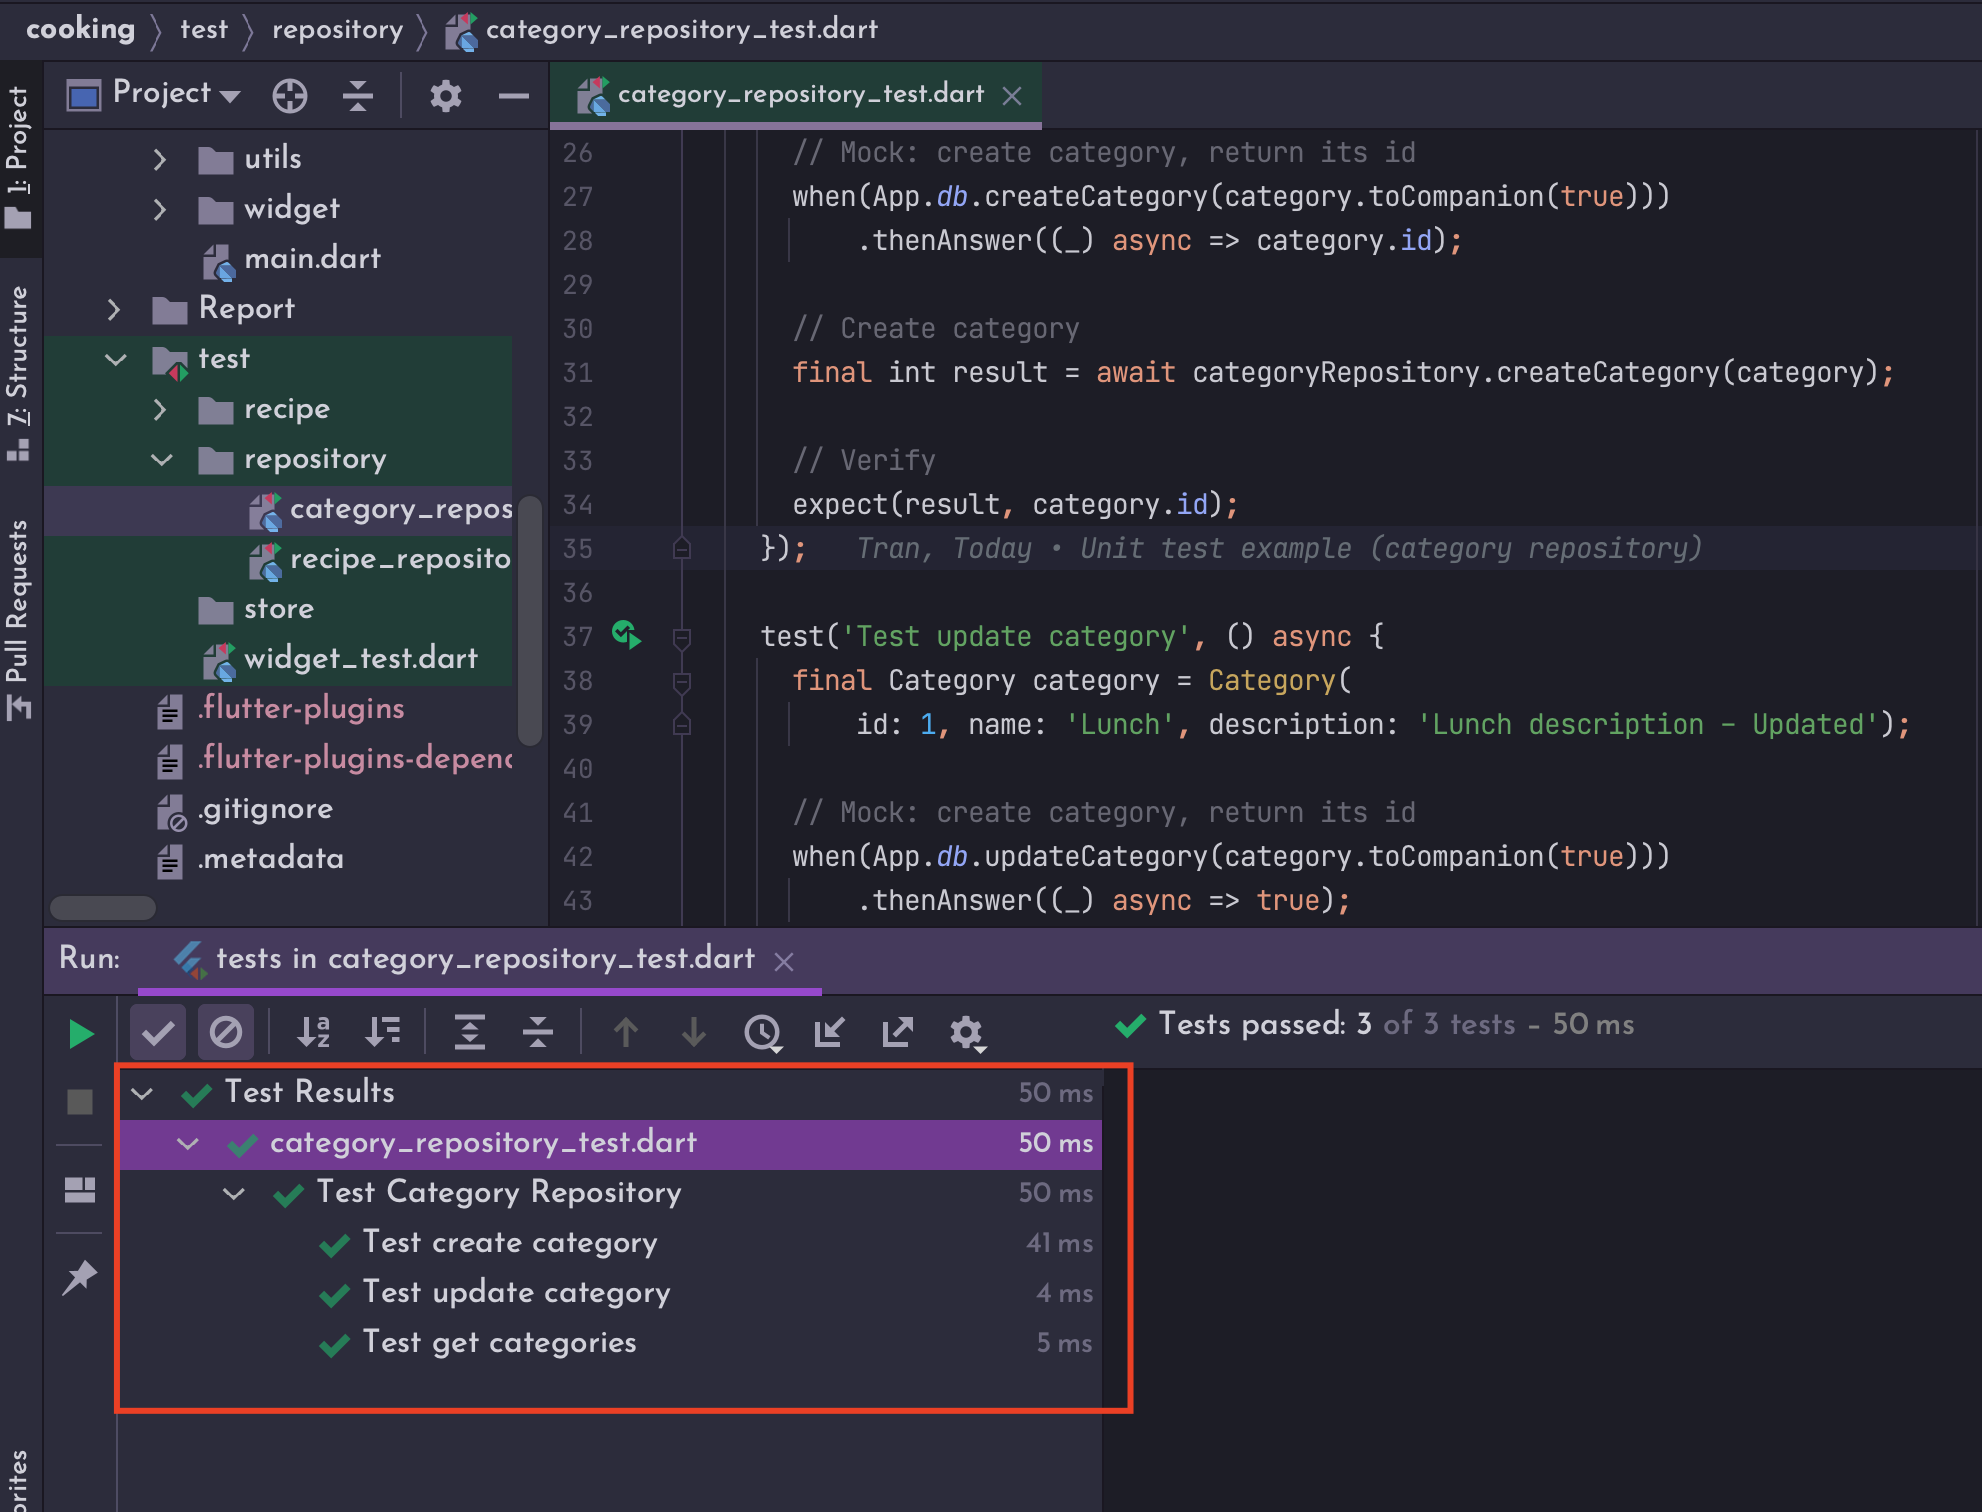
\includegraphics[scale=0.13]{Images/unit-test-for-recipe.png}
            \caption{Unit test for categories}
            \label{fig:cookingbook}
    \end{figure}
Unit test for recipe
    \begin{figure}[h!]
            \centering
            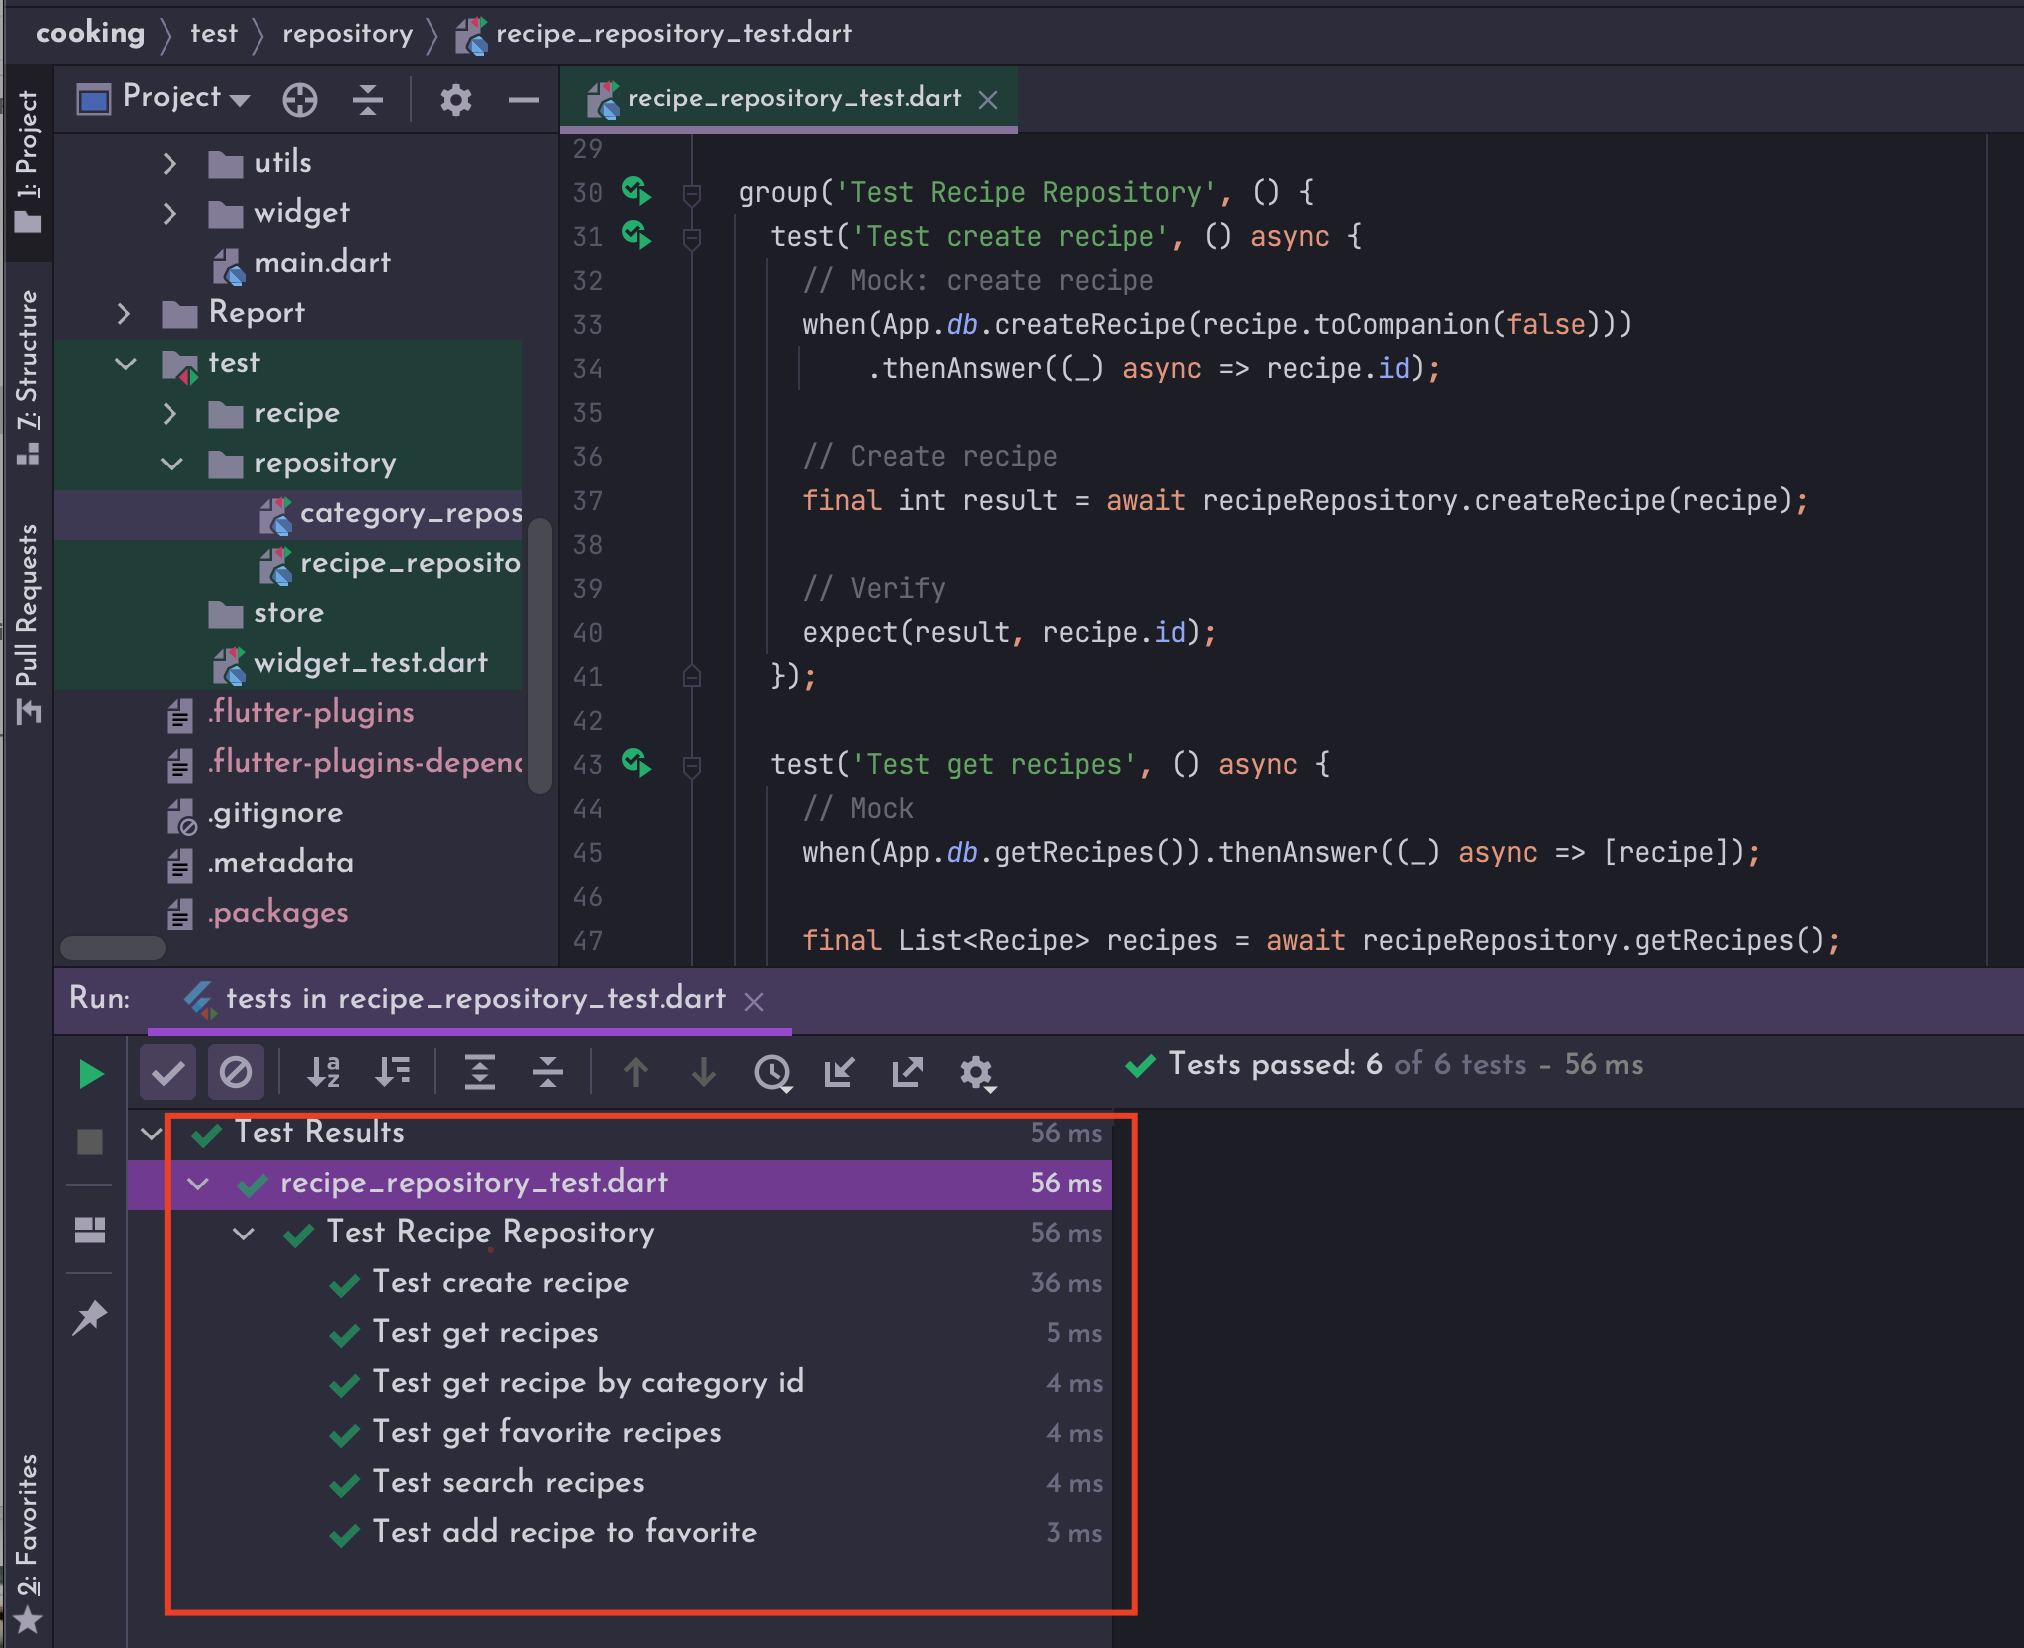
\includegraphics[scale=0.13]{Images/unit-test-repo.png}
            \caption{Unit test for recipe }
            \label{fig:cookingbook}
    \end{figure}
\newpage
    \subsubsection{EXPERIMENTS, SOME TESTS, SOME FIRST RELEASE} 
    For plan of development of team include 3 phases :   
    \begin{enumerate}
        \item \textbf{Phase 1 : 30 Jun 2020} : Initialize application with flutter code. As we need verify that team can work with new framework and technology, that we need try to new an empty app, and prepare all enviroments and tools for next step. On end of Jun, we have an empty app. \\
        \begin{figure}[h!]
            \centering
            
\includegraphics[scale=0.17]{Images/flashcreen.jpg}
            \caption{Version 0.1 for app - Just display fashscreen}
            \label{fig:cookingbook}
            \end{figure}
        \item \textbf{Phase 2 : 30 Jul 2020} : Initialize main function and architecture, so we need a plan on end of Jul 2020, all main architecture need to be implemented, all main screen need to initialize, ( home page, search recipe page, edit/add new recipe ). After that time, we have an application install file that can install in android with that install file all function are working, but test may not cover all function.\\
        \begin{figure}[h!]
        \centering
        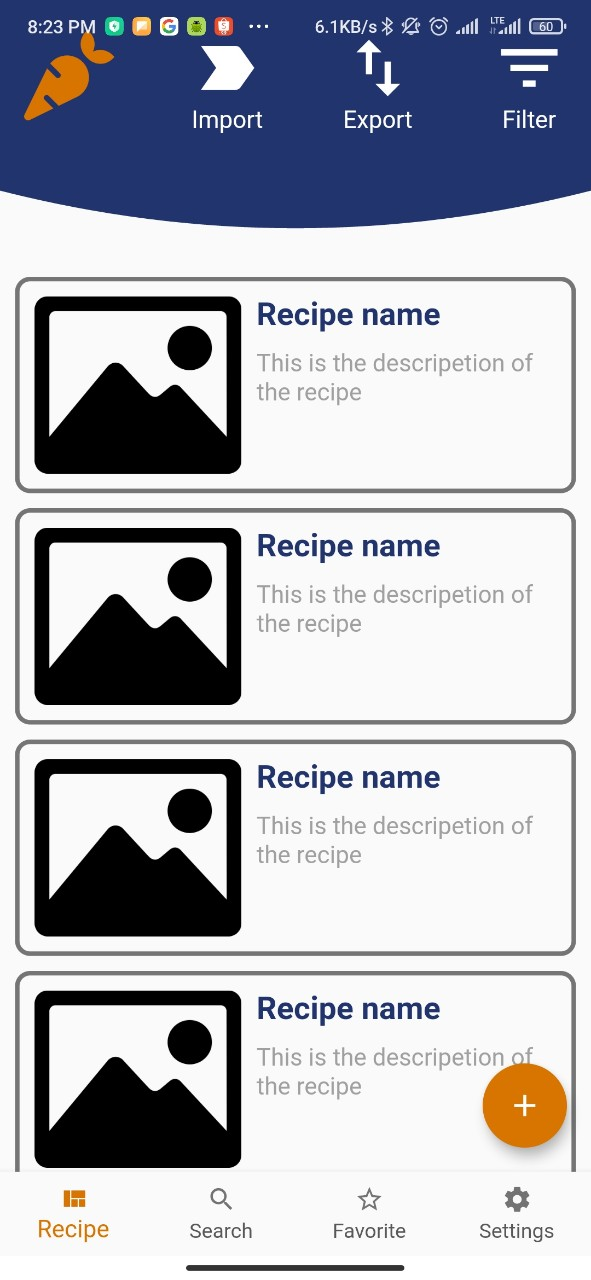
\includegraphics[scale=0.33]{Images/CookingBook.jpg}
        \caption{Version 1 for app}
        \label{fig:cookingbook}
        \end{figure}

        \item \textbf{Phase 3 : 30 Aug 2020} : Final for the rest function and test all function to make sure we can release it. On this phase, all Unit test need passed.
        \begin{figure}[h!]
        \centering
        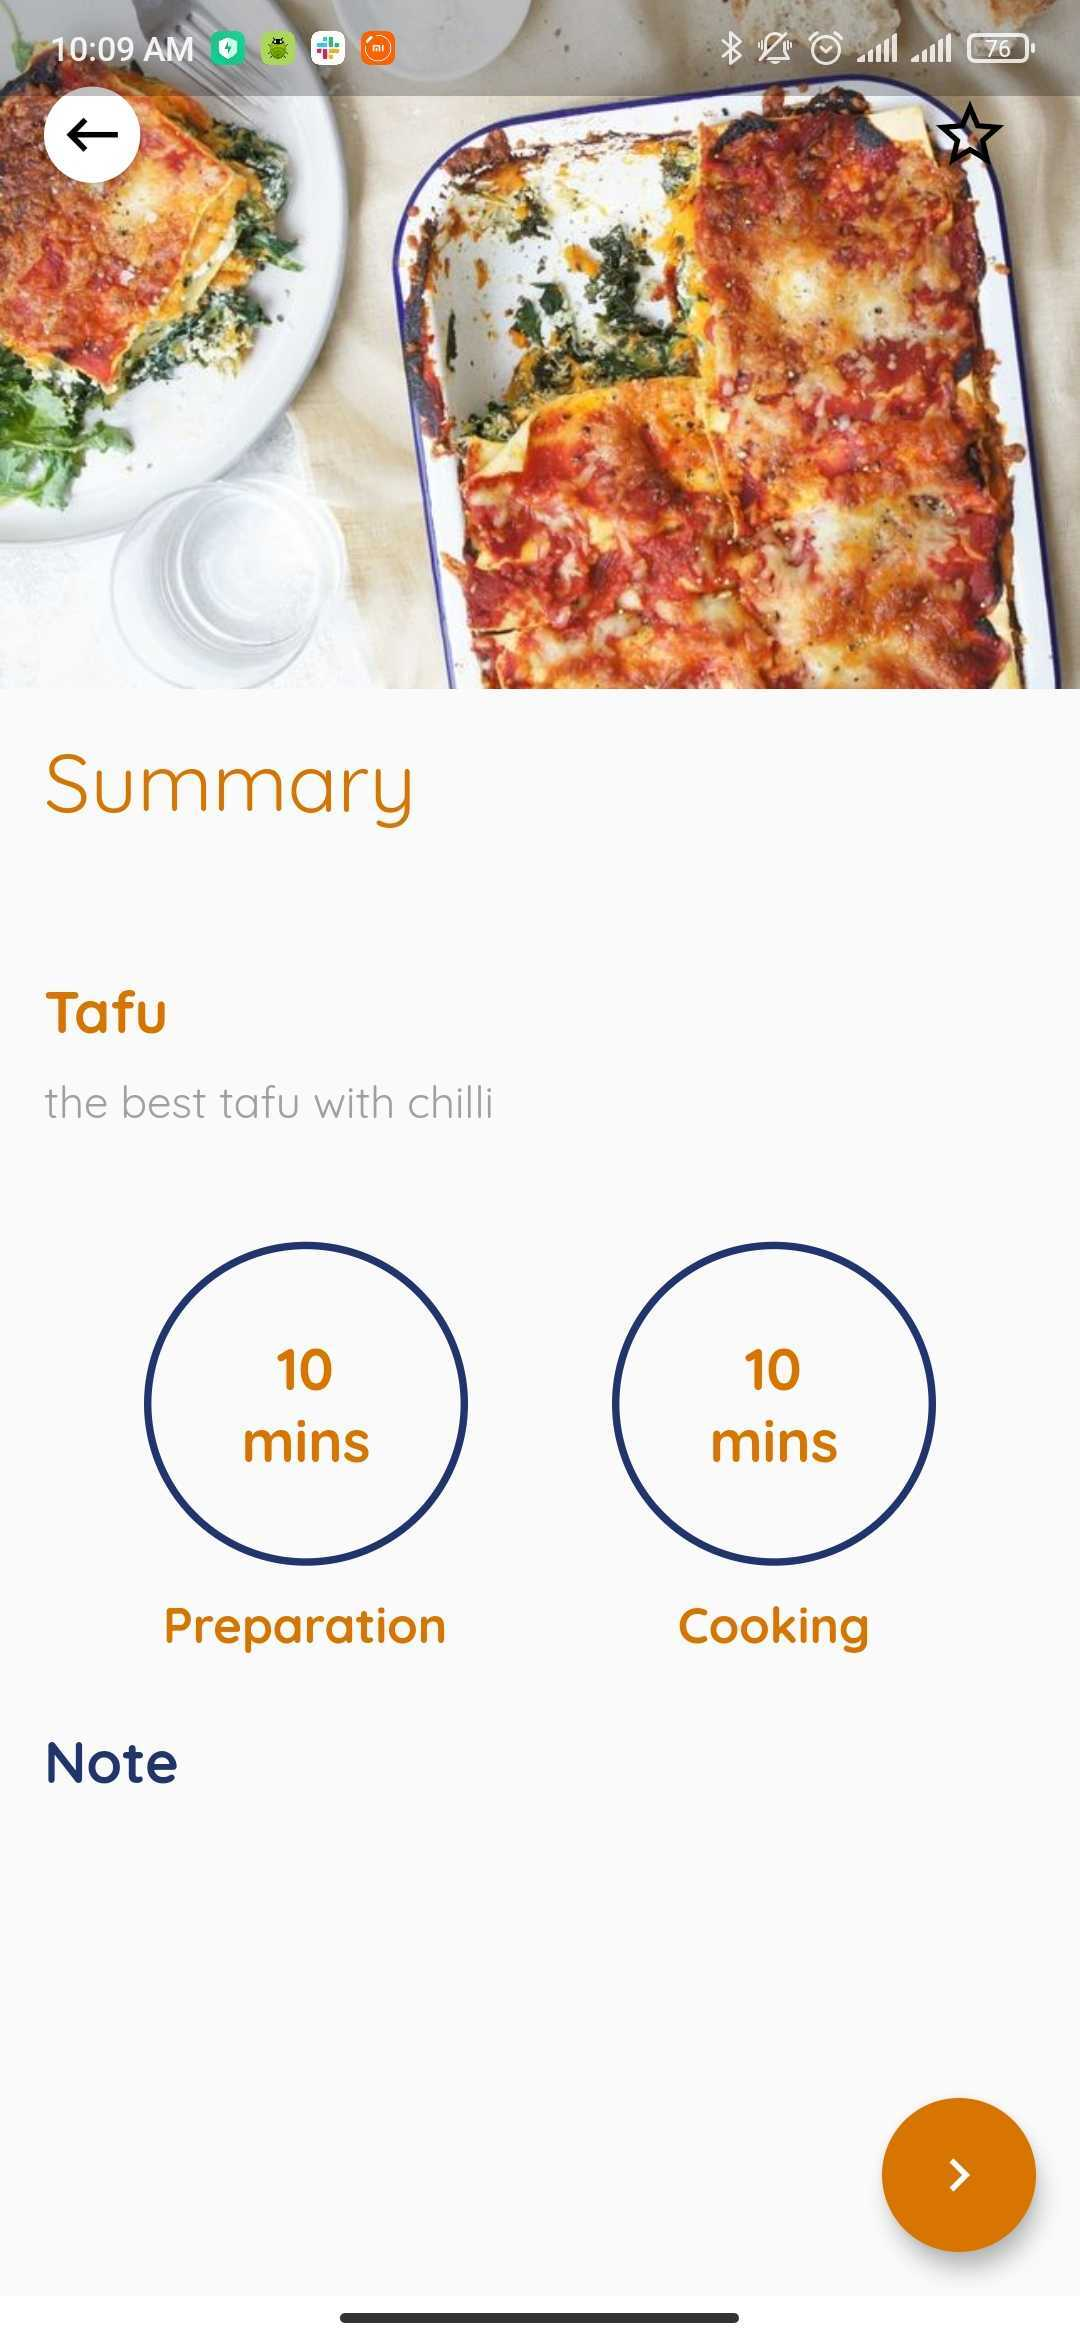
\includegraphics[scale=0.17]{Images/Homepage_data.jpg}
        \caption{Version 2 for app}
        \label{fig:cookingbook}
        \end{figure}
    \end{enumerate}
\newpage 
\subsubsection{RATIONALIZED DEVELOPMENT}
\begin{enumerate}
\item \textbf{IDE} : Intellij 
\item \textbf{Version control software}  : git , Git Repository : https://github.com/thphuc/cooking-app  . All member has their owns branch in local, but all working in dev branch.
\item \textbf{Builders} : Intellij build-in builder for flutter to build android and ios program.
\item \textbf{Debuggers} : Flutter DevTools - DevTools is a suite of performance and debugging tools for Dart and Flutter. It’s currently in beta release, but is under active development.\textbf{ What we can do with DevTools } : \\
-Inspect the UI layout and state of a Flutter app. \\
-Diagnose UI jank performance issues in a Flutter app. \\
-CPU profiling for a Flutter or Dart app. \\
-Network profiling for a Flutter app. \\
-Source-level debugging of a Flutter or Dart app. \\
-Debug memory issues in a Flutter or Dart command-line app. \\
-View general log and diagnostics information about a running Flutter or Dart command-line app. \\
-Analyze code and app size \\
-And many more ... \\
\item \textbf{Documentation} : Dartdoc - The \textbf{dartdoc} command creates API reference documentation from Dart source code.
\item \textbf{Tests} : Flutter support it's own testing library include 3 levels :  \\
-Unit test :  handy for verifying the behavior of a single function, method, or class. The \textbf{test} package provides the core framework for writing unit tests. \\
-Integration test : test how individual pieces work together as a whole ( Unit and Widget ), or capture the performance of an application running on a real device. These tasks are performed with integration tests.  The \textbf{flutter-driver} package provides the core framework for writing Integration tests \\
 -Widget test: handy for verifying the behavior of widget class . The \textbf{flutter-test} package provides the core framework for writing Widget tests. \\
On this project, we most focus on Unit Test only. It's supported from Flutter framework.
\item \textbf{Performance estimation and memory analysis} : Flutter DevTools - DevTools is a suite of performance and debugging tools for Dart and Flutter. It’s currently in beta release, but is under active development.
\end{enumerate}

\subsection{Scientific approach } 
\subsubsection{justify facts and choices (references, alternatives, tests, experiments)}
All the report included explain the solution, and reference .
\subsubsection{being rigorous during verification of the work done (tests, experiments)}
All function include Unit Test to make sure the program working well.
\subsubsection{knowing context and domain of application (bibliography, existing analysis)}
Please refer Requirement Analysis for more Details.
\subsubsection{write a documentation and confrontation of ideas}
Included in the report.

\section{Conclusion }
\qquad After developing a software product, the team realized that it not only involves writing software, but in that, in order to ensure the product quality, it takes a lot of work, and the team's support, from source code management, to writing documentation, or writing unit-tests to secure software products.
After the process, everyone on the team gained more experience in the process of producing a big software product.
\section{Appendix }
\end{document}